\documentclass[11pt,a4paper]{article}

% ------------------------------------------------------------------
%  XPP Studio: an introduction and tutorial
%  Compiles with pdfLaTeX (Overleaf default). Figures are in figures/.
% ------------------------------------------------------------------
\usepackage[utf8]{inputenc}
\usepackage[T1]{fontenc}
\usepackage{lmodern}
\usepackage{microtype}
\usepackage[margin=2.5cm]{geometry}
\usepackage{amsmath,amssymb}
\usepackage{graphicx}
\usepackage{booktabs}
\usepackage{tabularx}
\usepackage{xcolor}
\usepackage{tikz}
\usepackage{listings}
\usepackage[most]{tcolorbox}
\usepackage{enumitem}
\usepackage{caption}
\usepackage[hidelinks]{hyperref}

\graphicspath{{figures/}}

% Where the app lives. Change this if you share a different copy.
\newcommand{\xppurl}{https://claude.ai/artifact/GFisMVq8TzaNt5rN9cETpY}
\newcommand{\XS}{\textsf{XPP Studio}}
\newcommand{\XPP}{\textsf{XPPAUT}}
\newcommand{\ui}[1]{\textsf{\textbf{#1}}}          % a button, tab or menu
\newcommand{\key}[1]{\tikz[baseline=(k.base)]\node[draw,rounded corners=1.5pt,inner sep=1.6pt,font=\ttfamily\small](k){#1};}

\definecolor{codebg}{HTML}{F5F6F8}
\definecolor{codekw}{HTML}{1D4ED8}
\definecolor{codecm}{HTML}{6B7280}
\definecolor{tryc}{HTML}{1D4ED8}

\lstdefinelanguage{ode}{
  morekeywords={par,param,parameter,number,init,aux,wiener,markov,table,volterra,done,global,delay},
  sensitive=false,
  morecomment=[l]{\#},
  morestring=[b]",
}
\lstset{
  language=ode,
  basicstyle=\ttfamily\small,
  keywordstyle=\color{codekw}\bfseries,
  commentstyle=\color{codecm}\itshape,
  backgroundcolor=\color{codebg},
  frame=none,
  xleftmargin=6pt,xrightmargin=6pt,
  aboveskip=8pt,belowskip=8pt,
  columns=fullflexible,
  keepspaces=true,
  upquote=true,
  literate={-}{{-}}1,
}

\newtcolorbox{tryit}[1][]{enhanced,breakable,colback=tryc!4,colframe=tryc!55,
  boxrule=0.6pt,arc=2pt,left=6pt,right=6pt,top=4pt,bottom=4pt,
  title={\sffamily\bfseries Try it#1},fonttitle=\small,coltitle=white,colbacktitle=tryc!75}
\newtcolorbox{notebox}{enhanced,breakable,colback=black!3,colframe=black!25,boxrule=0.5pt,arc=2pt,
  left=6pt,right=6pt,top=4pt,bottom=4pt}

\setlist{itemsep=2pt,topsep=4pt}
\captionsetup{font=small,labelfont=bf}

\title{\XS\\[4pt]\large An introduction and tutorial}
\author{Peter Ashwin and Bard Ermentrout\\[2pt]
  \small with Claude Opus 5.5 (Anthropic)}
\date{October 2026}

\begin{document}
\maketitle

\begin{abstract}
\noindent \XS{} is a browser-based environment for exploring dynamical systems, modelled on Bard Ermentrout's \XPP{}. It reads \XPP{}'s \texttt{.ode} files and provides phase planes, three-dimensional views, time courses, numerical continuation of equilibria and periodic orbits, one- and two-parameter bifurcation diagrams, maps, stochastic and Markov models, stiff solvers, delay equations, events (global flags), arrays and Volterra integral equations. Everything runs locally in a web page: there is nothing to install and no data leaves the browser. This document introduces the interface, describes the model language, and works through a sequence of short tutorials using the examples that come with the program.
\end{abstract}

\tableofcontents
\newpage

% ==================================================================
\section{Introduction}

For more than thirty years \XPP{} \cite{ermentrout2002} has been one of the standard tools for simulating and analysing differential equations in mathematical biology, neuroscience and applied dynamical systems. Its strengths are a compact, readable model language, fast interactive phase-plane analysis, and a tight connection to the continuation package \textsf{AUTO} \cite{doedel2007}. \XS{} keeps that model language and that way of working, and puts them in a modern interface:

\begin{itemize}
  \item \textbf{Same files.} Most \XPP{} \texttt{.ode} files load unchanged. Supported features include parameters, functions, fixed quantities, auxiliary variables, maps, Wiener noise, Markov variables, tables, periodic (folded) variables, arrays, Volterra integrals, delays and global flags (Section~\ref{sec:language}).
  \item \textbf{Live analysis.} Dragging a parameter slider immediately recomputes trajectories, nullclines and equilibria.
  \item \textbf{Built-in continuation.} Equilibria, periodic orbits and their bifurcations can be continued in one or two parameters without leaving the program. Detected points include folds, Hopf, period-doubling, torus, fold-of-cycles and codimension-two points.
  \item \textbf{Publication output.} Every view can be exported as a vector SVG figure. Continuation data can be exported as CSV, and trajectories copied as CSV.
\end{itemize}

\noindent The program is a single web page. To use it, open
\begin{center}
  \url{\xppurl}
\end{center}
in any recent browser. (If the link has not been shared with you, ask the author for access, or open a local copy of the HTML file.)

\paragraph{How this document is organised.} Section~\ref{sec:tour} is a tour of the interface and Section~\ref{sec:language} summarises the model language. Sections~\ref{sec:pp}--\ref{sec:volterra} are hands-on tutorials, each built on an example from the \ui{Model} menu. Section~\ref{sec:numerics} covers numerical settings and Section~\ref{sec:export} exporting results. The document ends with the differences from \XPP{} and with credits.

% ==================================================================
\section{A tour of the interface}\label{sec:tour}

\begin{figure}[t]
  \centering
  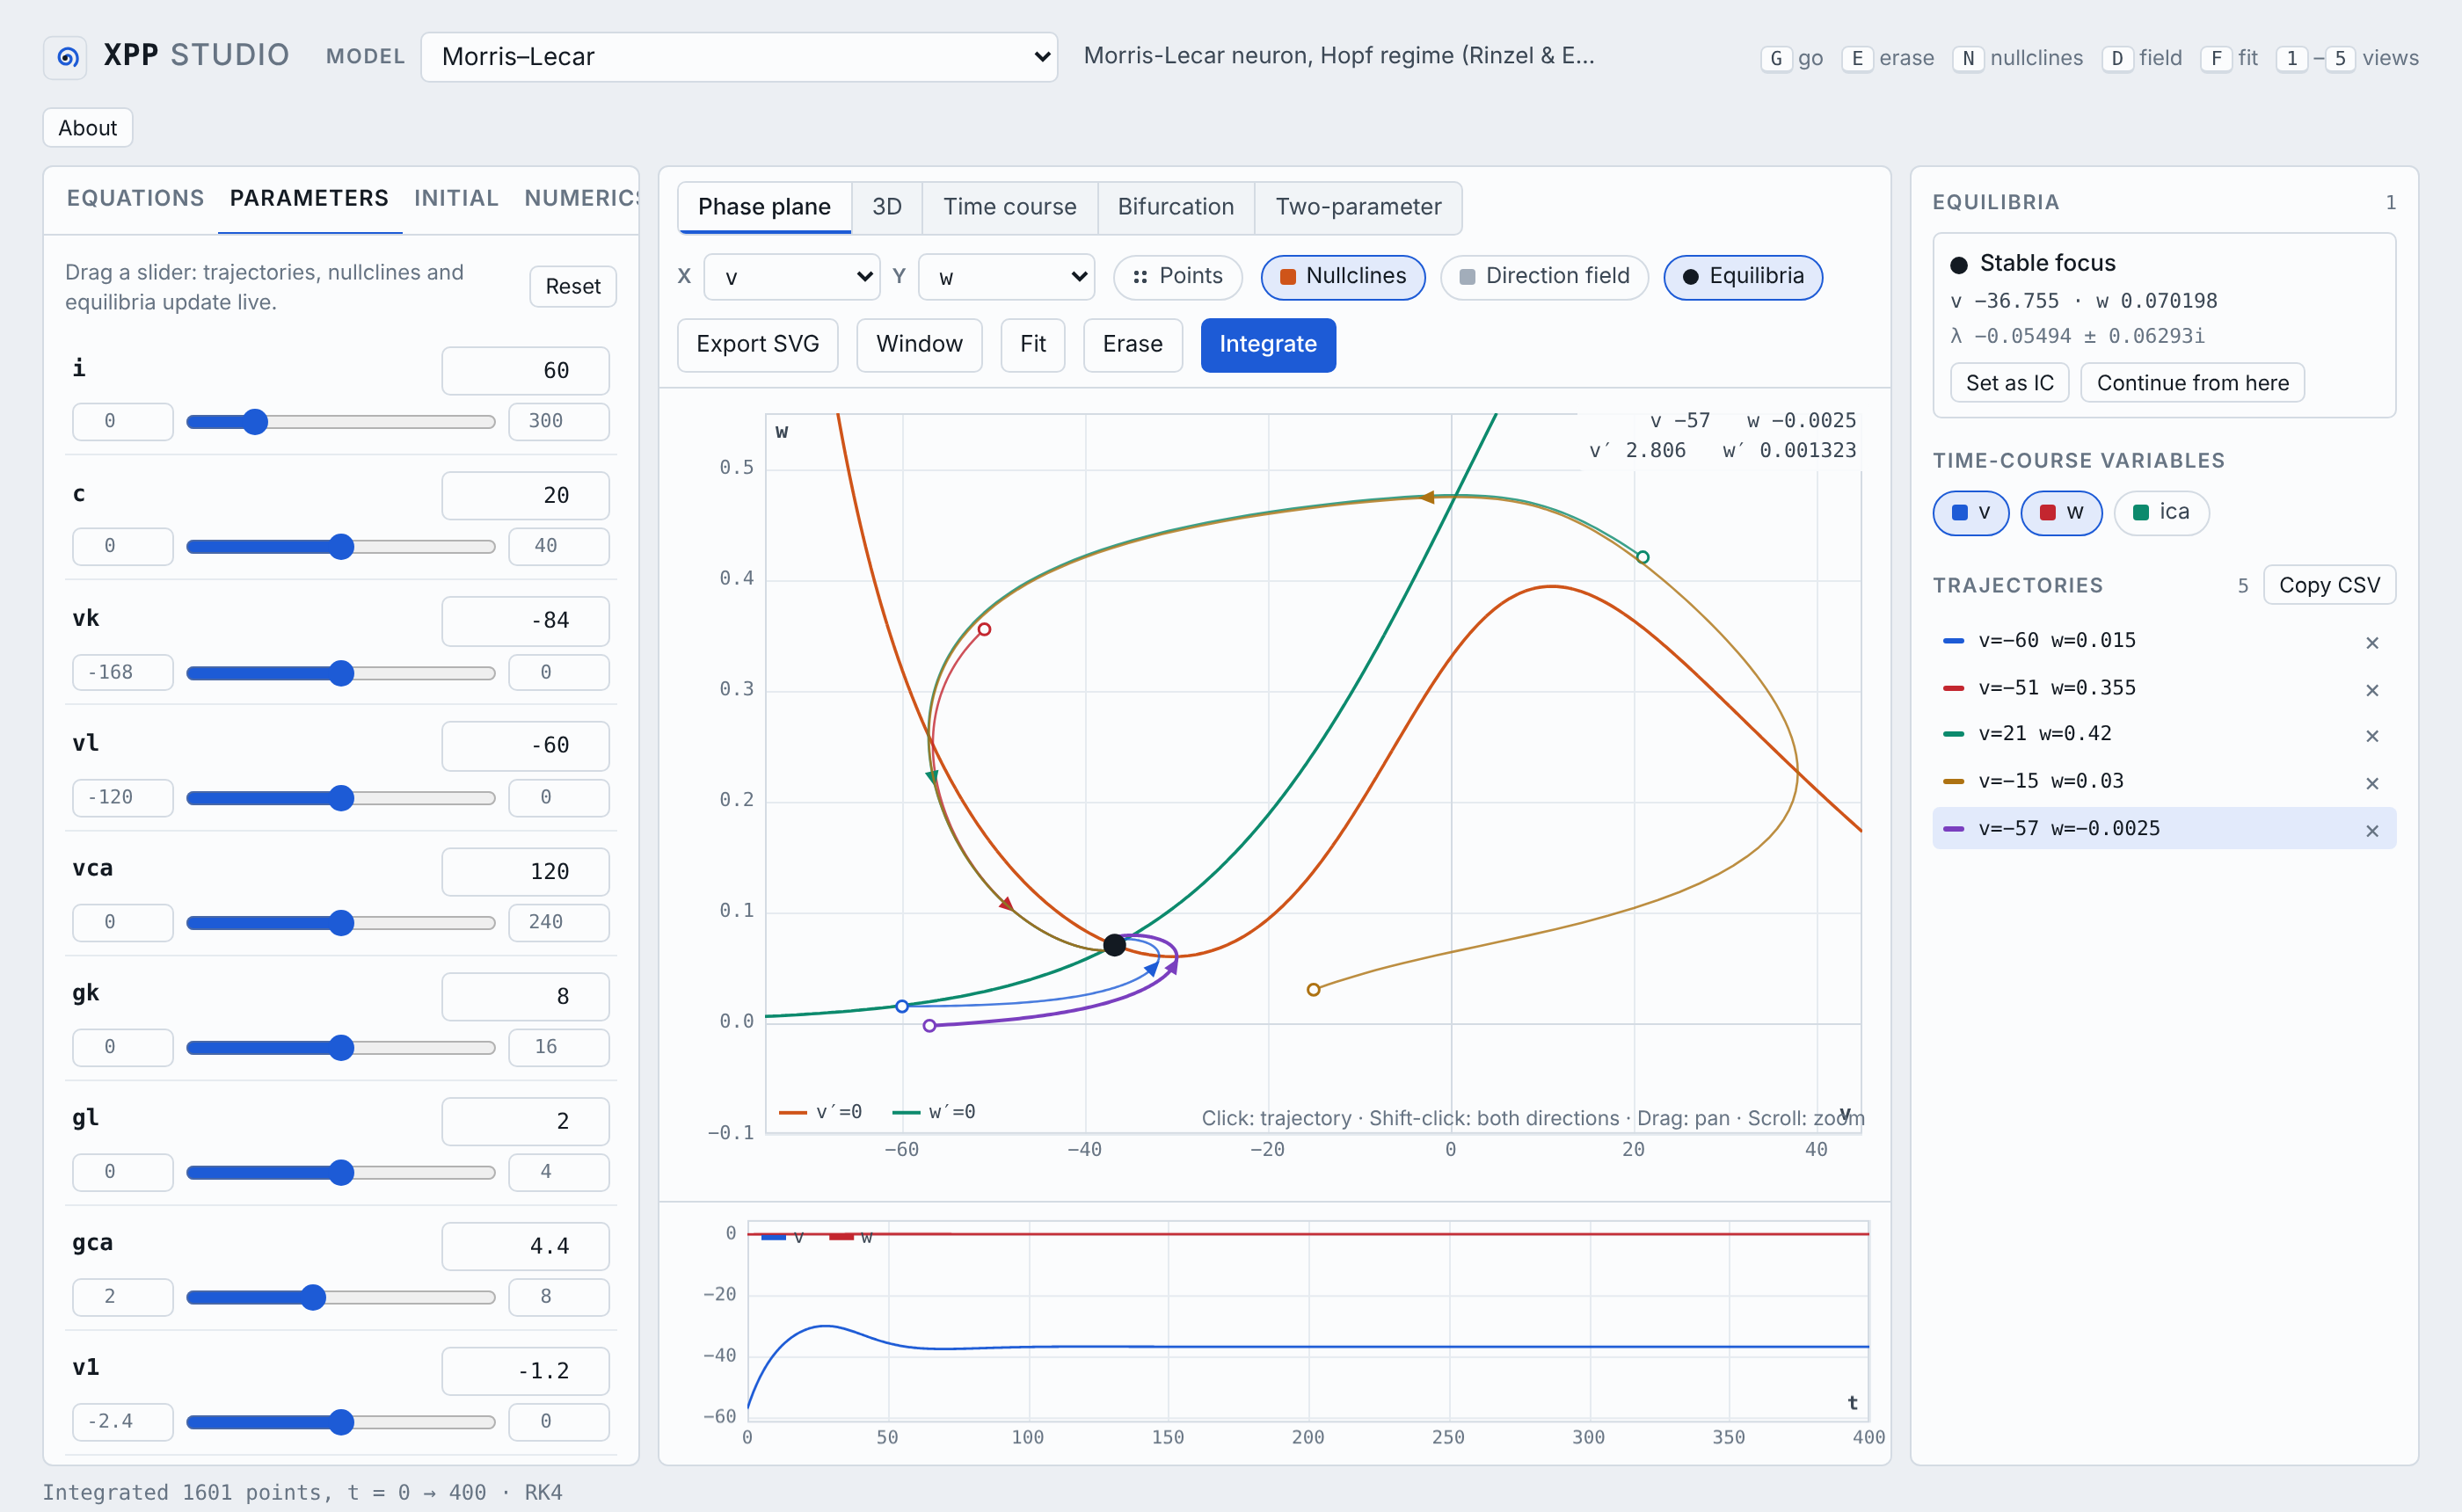
\includegraphics[width=\textwidth]{ui-overview.png}
  \caption{The \XS{} window with the Morris--Lecar example loaded. Left: tabs for equations, parameters, initial conditions and numerics. Centre: the plot, here the $(v,w)$ phase plane with nullclines, five trajectories and a stable focus, plus a time-course strip underneath. Right: the inspector, listing equilibria, the variables shown in the time course, and the trajectories.}
  \label{fig:overview}
\end{figure}

The window (Figure~\ref{fig:overview}) has three columns.

\paragraph{Left: the model.} Four tabs:
\begin{description}[font=\sffamily\bfseries]
  \item[Equations] The \texttt{.ode} text, which you can edit freely. \ui{Apply} (or \key{Ctrl}+\key{Enter}) reloads the model, and messages underneath report what was loaded and any errors, with line numbers. \ui{Open .ode} loads a file from disk, \ui{Copy text} copies the current text, \ui{Write state} writes the current parameters, initial conditions and settings into it (Section~\ref{sec:writestate}), and \ui{Table files} supplies data files used by \texttt{table} declarations.
  \item[Parameters] One row per parameter, with a value box and a slider whose limits you can edit. Drag a slider to see everything update live, and use \ui{Reset} to restore the values in the file.
  \item[Initial] Initial values of the state variables (and Markov states). \ui{Integrate} runs from here, and \ui{Last point $\to$ IC} copies the end of the current trajectory into the initial conditions.
  \item[Numerics] Integration method, total time, transient, step size, tolerance and bound, plus the continuation settings (Section~\ref{sec:numerics}).
\end{description}

\paragraph{Centre: the plot.} Five views, chosen with the buttons above the plot or with the keys \key{1}--\key{5}:
\begin{description}[font=\sffamily\bfseries]
  \item[Phase plane] Any two variables (state, Markov, Volterra or auxiliary) against each other, with optional nullclines, direction field and equilibria. For a one-dimensional map this view shows a cobweb diagram.
  \item[3D] Three variables (or time) in a rotatable box: drag to rotate, scroll to zoom, \ui{Spin} to animate.
  \item[Time course] Chosen variables against $t$ (or the iteration number $n$ for maps).
  \item[Bifurcation] Branches of equilibria and periodic orbits, and parameter sweeps, against one parameter.
  \item[Two-parameter] Curves of folds, Hopf points, period doublings and bifurcations of cycles in a parameter plane.
\end{description}
In every view you drag to pan and scroll to zoom. \ui{Fit} rescales to the data, and \ui{Window} sets the axis limits by hand (they then stay fixed until you press \ui{Fit}). \ui{Points} draws trajectories as dots instead of lines, which is the default for maps. \ui{Export SVG} saves the current view as a vector figure. In the Bifurcation and Two-parameter views, \ui{Export CSV} saves the computed data.

\paragraph{Right: the inspector.} The inspector's contents depend on the view. In the phase plane it lists the equilibria (type, coordinates and eigenvalues, with buttons to make one the initial condition, start continuation from it, or draw its separatrices), the variables in the time course, and the trajectories. In the Bifurcation view it holds the continuation controls and the table of special points. In the Two-parameter view it holds the two-parameter controls.

\begin{table}[h]
\centering\small
\begin{tabular}{@{}ll@{}}
\toprule
Key & Action\\
\midrule
\key{G} & integrate from the current initial condition (``go'')\\
\key{E} & erase all trajectories\\
\key{N} / \key{D} & toggle nullclines / direction field\\
\key{F} & fit the axes to the data\\
\key{1}--\key{5} & phase plane, 3D, time course, bifurcation, two-parameter\\
\key{Esc} & during continuation: skip to the other direction (``soft interrupt'')\\
\key{Shift}+\key{Esc} & stop the continuation altogether\\
click / shift-click & start a trajectory (shift: forwards and backwards in time)\\
\bottomrule
\end{tabular}
\caption{Keyboard shortcuts and mouse actions.}
\end{table}

% ==================================================================
\section{The model language}\label{sec:language}

A model is a plain-text \texttt{.ode} file in \XPP{}'s format. Lines starting with \texttt{\#} are comments, and the first comment line becomes the model's title. Names are case-insensitive. The Morris--Lecar example \cite{morris1981,rinzel1989} illustrates most of the basic syntax:

\begin{lstlisting}
# Morris-Lecar neuron, Hopf regime (Rinzel & Ermentrout)
dv/dt=(i+gl*(vl-v)+gk*w*(vk-v)+gca*minf(v)*(vca-v))/c
dw/dt=phi*(winf(v)-w)/tauw(v)
minf(v)=.5*(1+tanh((v-v1)/v2))
winf(v)=.5*(1+tanh((v-v3)/v4))
tauw(v)=1/cosh((v-v3)/(2*v4))
aux ica=gca*minf(v)*(v-vca)
param i=60,c=20
param vk=-84,vl=-60,vca=120
param gk=8,gl=2,gca=4.4
param v1=-1.2,v2=18,v3=2,v4=30,phi=.04
init v=-60,w=0.015
#@range i 0 300
@ total=400,dt=0.25,meth=rk4,xp=v,yp=w
@ xlo=-75,xhi=45,ylo=-0.1,yhi=0.55
done
\end{lstlisting}

\noindent Table~\ref{tab:syntax} summarises the language. The \texttt{\#@range} line is an \XS{} extension that sets a slider's range. Because it starts with \texttt{\#}, \XPP{} reads it as a comment, so files stay portable.

\begin{table}[p]
\centering\small
\renewcommand{\arraystretch}{1.15}
\begin{tabularx}{\textwidth}{@{}>{\ttfamily}p{0.40\textwidth}X@{}}
\toprule
\normalfont Syntax & Meaning\\
\midrule
x'=\ldots\ \ or\ \ dx/dt=\ldots & differential equation\\
x(t+1)=\ldots & map (or use \texttt{x'=\ldots} with \texttt{@ meth=discrete})\\
x(0)=1\ \ or\ \ init x=1,y=0 & initial values\\
par a=1, b=2 & parameters (also \texttt{param}, \texttt{p})\\
number c=3 & named constant\\
!d=a*b & derived parameter, recomputed when parameters change\\
f(x,y)=\ldots & user function\\
q=\ldots & fixed quantity, evaluated before the equations\\
aux s=\ldots & auxiliary output, plotted like a variable\\
wiener w & white noise for an SDE, e.g.\ \texttt{x'=-x+s*w}\\
markov z 2 \quad\{0\} \{kon\} \quad \{koff\} \{0\} & two-state Markov variable; entry $(i,j)$ is the rate from $i$ to $j$\\
table h \% 101 0 6.283 sin(t) & table sampled from an expression\\
table h data.tab & table read from a file (add it with \ui{Table files})\\
x[1..20]'=-x[j]+x[j-1] & array: the line is repeated for $j=1,\ldots,20$\\
\%[1..20] \ldots\ \% & repeat a block of lines\\
int\{K(t,t',x)\} & Volterra integral $\int_0^t K(t,t',x(t'))\,dt'$\\
int\{K\#x\} & convolution $\int_0^t K(t-t')\,x(t')\,dt'$\\
int[mu]\{\ldots\} & weakly singular kernel, extra factor $(t-t')^{-\mu}$\\
u(t)=\ldots int\{\ldots\} & integral equation (also \texttt{volterra u=\ldots})\\
delay(x,tau) & delayed value $x(t-\tau)$; $\tau$ may depend on the state\\
x(0)=0.5+0.2*cos(t) & history of a delay equation for $t<0$ (its value at $t=0$ is the initial condition)\\
global 1 x-1 \{x=0;y=y+1\} & global flag: when \texttt{x-1} crosses zero upwards (1), downwards ($-1$) or either way (0), make the assignments; \texttt{arret=1} stops the run\\
\#@range p lo hi & slider range for parameter \texttt{p}\\
\midrule
@ total, trans, dt, meth, toler, bound & integration: duration, transient, step, method, tolerance, bound\\
@ xp, yp, zp, axes=3, xlo, xhi, ylo, yhi & initial plot variables and window\\
@ fold=th, tor\_per=6.2832 & periodic variable \texttt{th} with the given period\\
@ seed=7 & fix the random seed\\
@ vmaxpts=4000 & memory length for Volterra integrals\\
@ ds, dsmin, dsmax, nmax, ntst, parmin, parmax & continuation numerics, as in \XPP{}'s \textsf{AUTO} window\\
\midrule
\multicolumn{2}{@{}p{\dimexpr\textwidth\relax}@{}}{\normalfont Functions: \texttt{sin cos tan exp ln log sqrt abs heav sign max min mod atan2 sinh cosh tanh}, \texttt{if(c)then(a)else(b)}, \ldots}\\
\bottomrule
\end{tabularx}
\caption{The \texttt{.ode} language understood by \XS{}.}
\label{tab:syntax}
\end{table}

\begin{notebox}
\textbf{Methods.} \texttt{meth=} accepts \texttt{rk4} (fixed-step Runge--Kutta), \texttt{euler}, \texttt{dp45} (adaptive Dormand--Prince 4(5)), and the stiff names \texttt{stiff}, \texttt{gear}, \texttt{cvode}, \texttt{rosenbrock} and \texttt{backeul}. All of the stiff names select an adaptive Rosenbrock 2(3) solver \cite{shampine1997}. \texttt{discrete} iterates a map. Models with Wiener variables always use Euler--Maruyama, and models with Volterra integrals use a product-trapezoid scheme.
\end{notebox}

% ==================================================================
\section{Tutorial 1: phase-plane analysis}\label{sec:pp}

\begin{figure}[t]
  \centering
  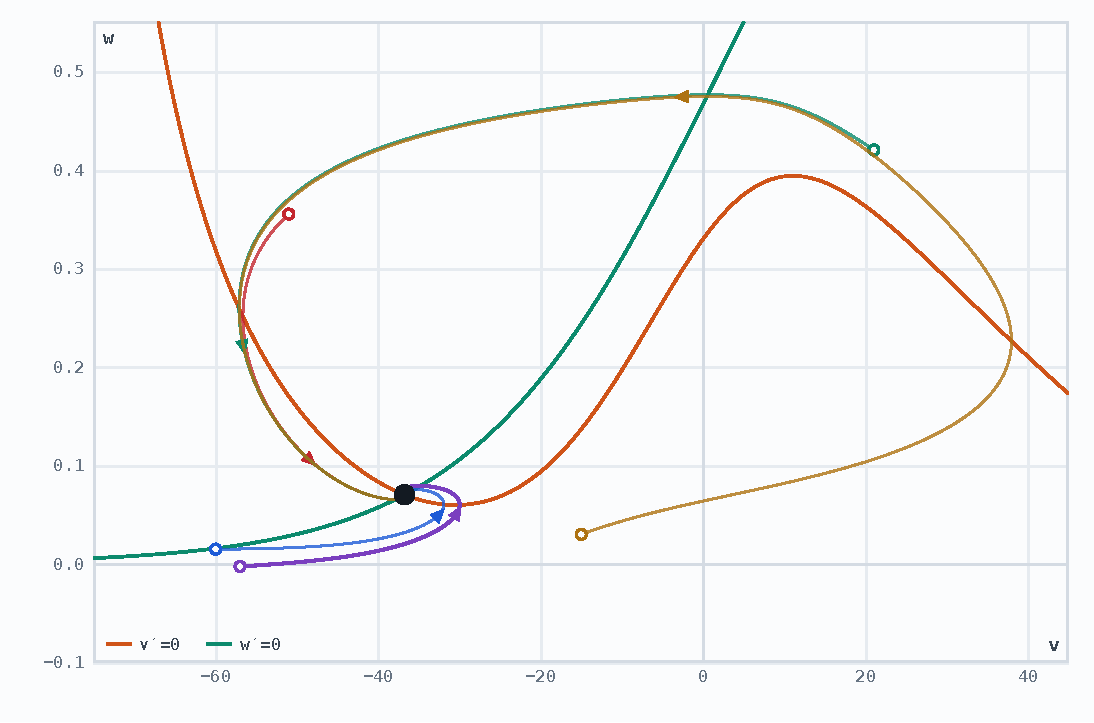
\includegraphics[width=0.75\textwidth]{ml-phaseplane.pdf}
  \caption{Morris--Lecar phase plane at $i=60$: the $v$-nullcline (orange), the $w$-nullcline (green), a stable focus (filled circle) and several trajectories. Open circles mark starting points.}
  \label{fig:mlpp}
\end{figure}

Choose \ui{Morris--Lecar} from the \ui{Model} menu. The phase plane shows $w$ against the membrane potential $v$, together with the two nullclines.

\begin{tryit}
\begin{enumerate}
  \item Click anywhere in the plane to start a trajectory there. Shift-click integrates both forwards and backwards. Each new trajectory gets its own colour and appears in the \ui{Trajectories} list, where you can remove it with~$\times$.
  \item Press \key{D} for the direction field and \key{N} to hide or show the nullclines. Hovering over the plot shows the coordinates and the derivatives $v'$, $w'$ at the pointer.
  \item The inspector lists one equilibrium, a \emph{stable focus}, with its eigenvalues $\lambda\approx-0.055\pm0.063i$. \ui{Set as IC} moves the initial condition onto it.
  \item Open the \ui{Parameters} tab and slowly drag the slider for the applied current~$i$. Between about $i=94$ and $i=212$ the focus becomes unstable and trajectories settle onto a large limit cycle: repetitive firing.
  \item Press \key{3} for the time course. The chips in the inspector choose which variables are plotted, auxiliary ones included (\texttt{ica} here).
\end{enumerate}
\end{tryit}

\noindent Equilibria are found by Newton's method from a grid of starting points covering the visible window, so panning or zooming out searches a wider region. For a saddle, the \ui{Separatrices} button integrates its stable and unstable manifolds.

% ==================================================================
\section{Tutorial 2: one-parameter bifurcation diagrams}\label{sec:bif}

\begin{figure}[t]
  \centering
  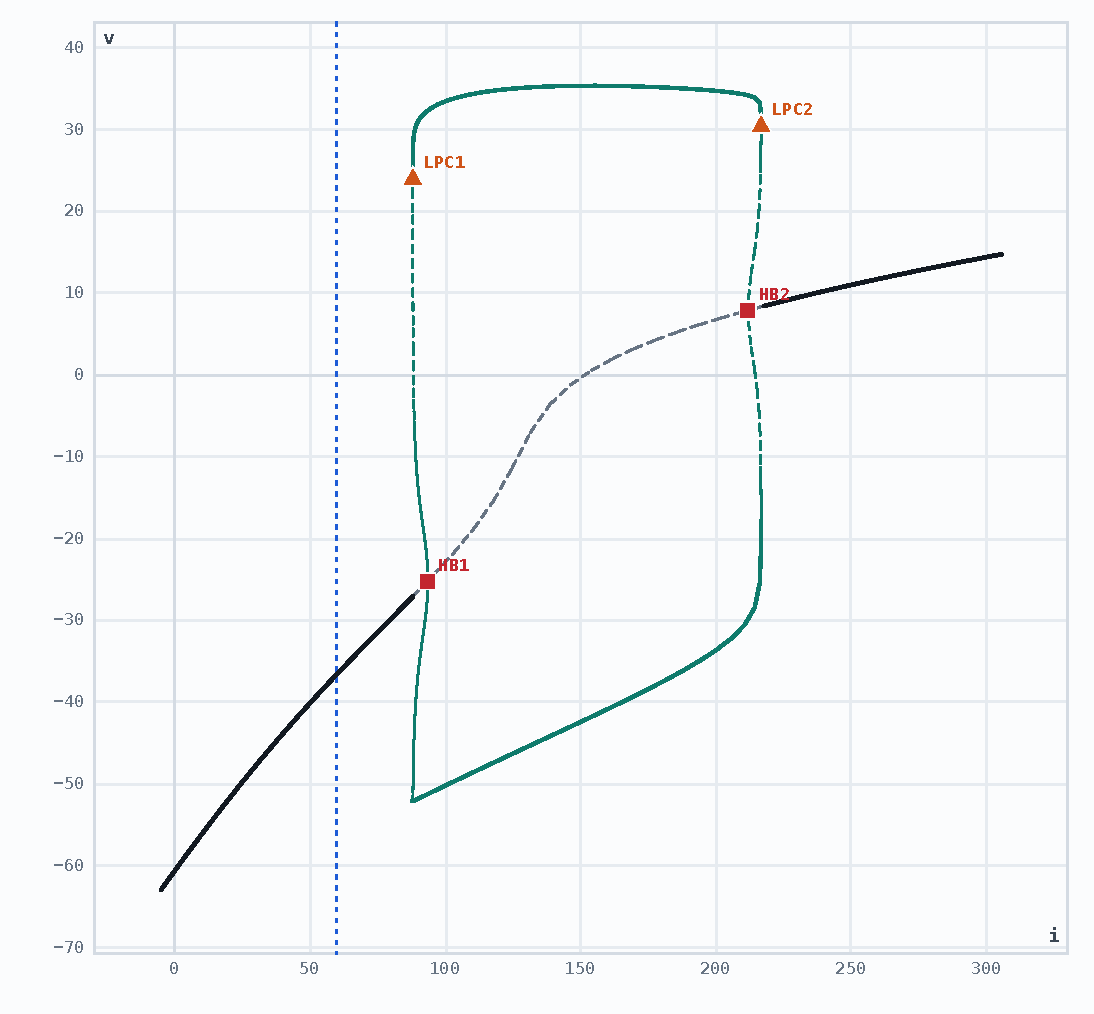
\includegraphics[width=0.72\textwidth]{ml-bifurcation.pdf}
  \caption{Bifurcation diagram of Morris--Lecar in the current~$i$. Black: equilibria (solid stable, dashed unstable). Green: maximum and minimum of $v$ along the periodic orbits born at the two Hopf points HB1 and HB2. Both Hopf bifurcations are subcritical. The orbit family turns at two folds of cycles, LPC1 and LPC2, giving bistability between rest and firing.}
  \label{fig:mlbif}
\end{figure}

Press \key{4} for the Bifurcation view. The inspector shows the continuation controls: the \ui{Parameter} to vary, the variable to \ui{Plot}, the parameter \ui{Range}, the initial step \ui{Step ds}, and the equilibrium to \ui{Start} from.

\begin{tryit}
\begin{enumerate}
  \item Press \ui{Continue equilibria}. Pseudo-arclength continuation \cite{keller1977} traces the branch in both directions across the range. Stability is read off the eigenvalues, and two Hopf points appear: HB1 at $i\approx 93.68$ (period $\approx 79.2$) and HB2 at $i\approx 212.06$. Each Hopf point is tagged \emph{sub} or \emph{super} in the \ui{Special points} table (Figure~\ref{fig:special}). The tag comes from the sign of the first Lyapunov coefficient $\ell_1$, and hovering over it shows the value. Both points here are subcritical ($\ell_1>0$), so the orbits born there are unstable.
  \item In the \ui{Special points} table, press \ui{Cycles} on the row for HB1. The periodic orbits born there are computed by multiple shooting with an integral phase condition, as in \textsf{AUTO}, and their stability comes from Floquet multipliers. While the computation runs, \key{Esc} (or \ui{Skip direction}) abandons the current direction and moves on, and \key{Shift}+\key{Esc} stops altogether.
  \item The family of orbits connects HB1 to HB2 and turns at two folds of cycles: LPC1 at $i\approx 88.29$ and LPC2 at $i\approx 216.90$ (Figure~\ref{fig:mlbif}). Between LPC1 and HB1 a stable orbit and the stable rest state coexist.
  \item Click any point of a branch to jump there. This sets the parameter and loads that equilibrium, or exactly one period of that orbit, as the current state. Clicking a row of the special-points table does the same.
  \item \ui{Limit cycle} starts orbit continuation from the current trajectory instead. Integrate onto a stable cycle first (e.g.\ at $i=150$), then press it.
\end{enumerate}
\end{tryit}

\noindent \ui{Sweep max/min} provides a brute-force alternative. It integrates at a grid of parameter values, carrying the end state forward, and plots every local maximum and minimum after the transient. This is the right tool for chaotic or stochastic regimes, where continuation does not apply (Tutorial~4).

\begin{figure}[h]
  \centering
  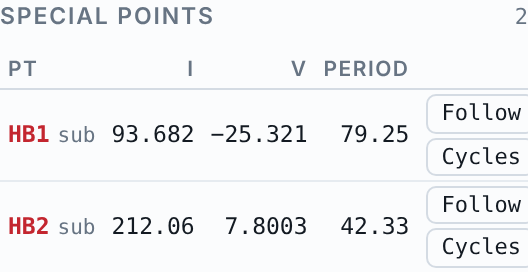
\includegraphics[width=0.55\textwidth]{ui-special.png}
  \caption{The \ui{Special points} table after continuing equilibria of Morris--Lecar. Both Hopf points are tagged \emph{sub} (subcritical). \ui{Follow} continues a point in two parameters, and \ui{Cycles} continues the periodic orbits born there.}
  \label{fig:special}
\end{figure}

\begin{notebox}
\textbf{Sub- or supercritical?} At a Hopf point with eigenvalues $\pm i\omega$, \XS{} computes the first Lyapunov coefficient
\[
\ell_1=\frac{1}{2\omega}\,\mathrm{Re}\Bigl[\langle p,C(q,q,\bar q)\rangle-2\langle p,B(q,A^{-1}B(q,\bar q))\rangle+\langle p,B(\bar q,(2i\omega I-A)^{-1}B(q,q))\rangle\Bigr],
\]
where $A$ is the Jacobian, $Aq=i\omega q$, $A^{\mathsf T}p=-i\omega p$ and $\langle p,q\rangle=1$ \cite{kuznetsov2004}. The multilinear forms $B$ and $C$ (the second and third derivatives of the vector field) are evaluated by finite differences. If $\ell_1<0$ the bifurcation is \emph{supercritical}: a small stable orbit appears on the side where the equilibrium is unstable. If $\ell_1>0$ it is \emph{subcritical}: an unstable orbit appears on the side where the equilibrium is stable, and the system usually jumps to a distant attractor.
\end{notebox}

\begin{notebox}
\textbf{What is detected.} For equilibria of flows: folds (LP), Hopf points (HB, tagged sub- or supercritical) and branch points (BP). For periodic orbits: folds of cycles (LPC), period doublings (PD) and torus (Neimark--Sacker) points (TR). For fixed points of maps: LP, PD and Neimark--Sacker (NS). At a PD of cycles, \ui{Double} switches to the period-doubled branch.
\end{notebox}

% ==================================================================
\section{Tutorial 3: two-parameter continuation}\label{sec:tp}

\begin{figure}[t]
  \centering
  \begin{minipage}[b]{0.56\textwidth}\centering
    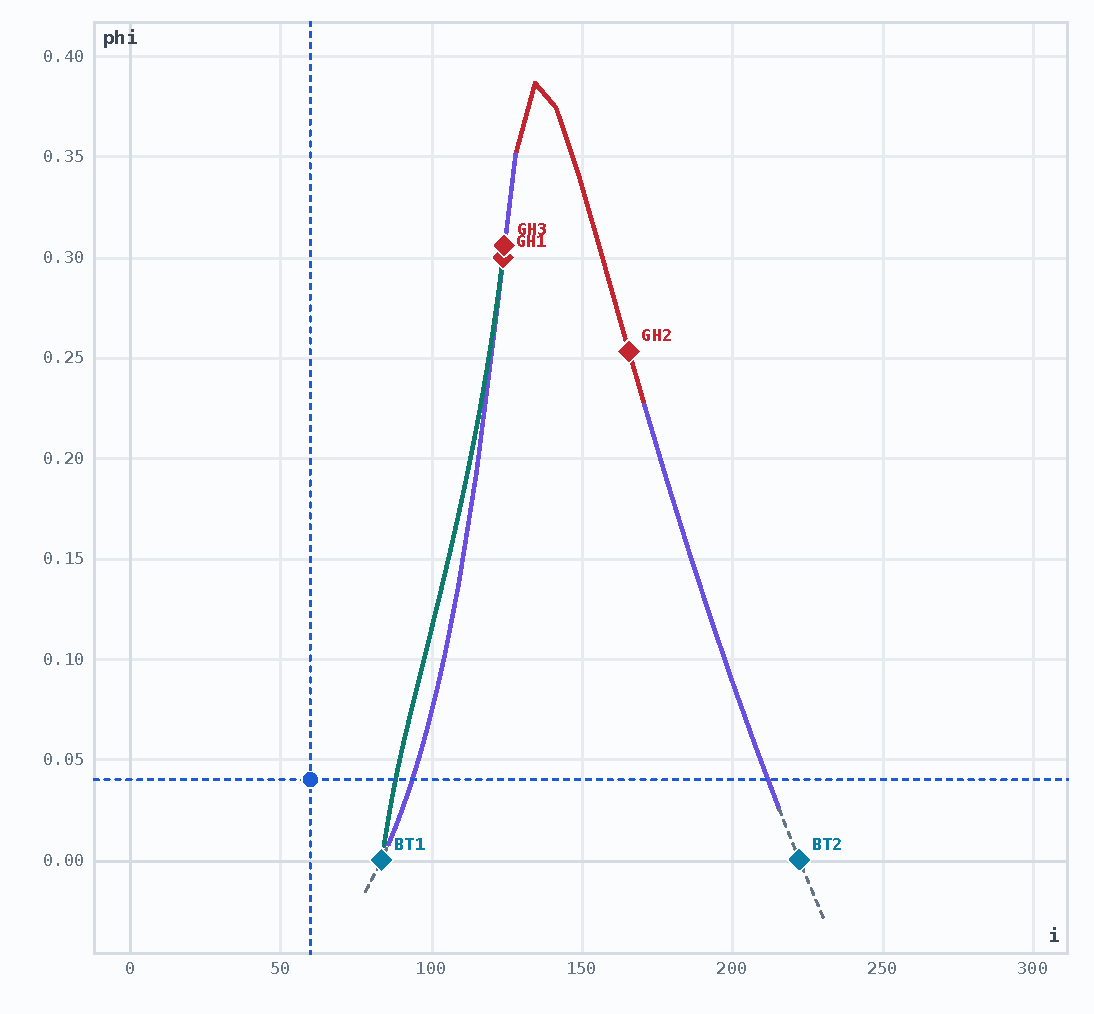
\includegraphics[width=\textwidth]{ml-twopar.pdf}
  \end{minipage}\hfill
  \begin{minipage}[b]{0.41\textwidth}\centering
    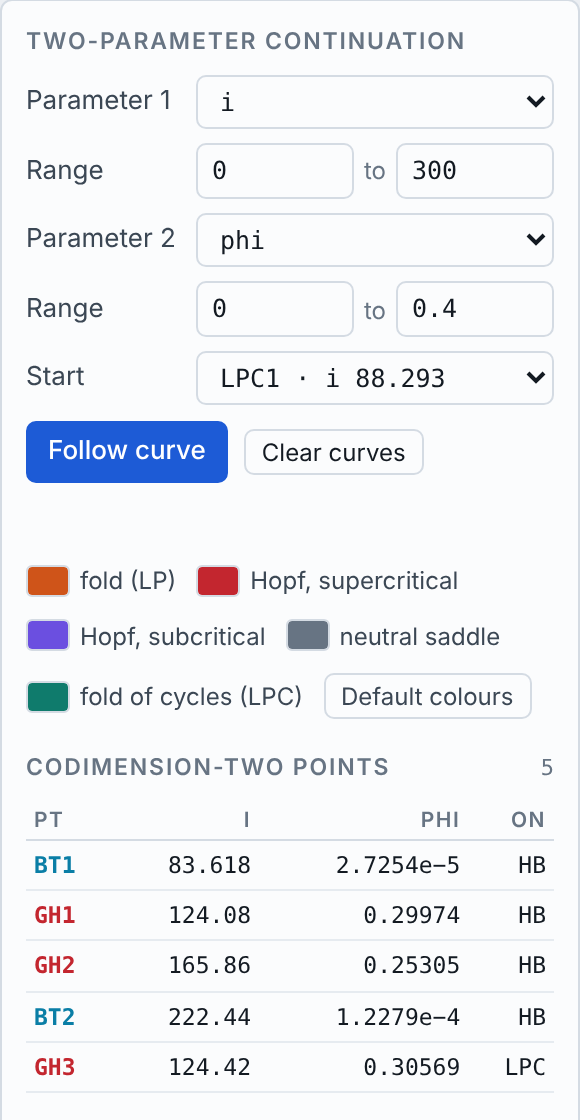
\includegraphics[width=\textwidth]{ui-twopar.png}
  \end{minipage}
  \caption{Left: two-parameter diagram for Morris--Lecar in $(i,\phi)$. A single Hopf curve joins HB1 and HB2. It is purple where the Hopf bifurcation is subcritical and red where it is supercritical, and the colour changes at the generalised Hopf (Bautin) points GH1 and GH2. Dashed ends are neutral saddles beyond the Bogdanov--Takens points BT1 and BT2 near $\phi=0$. The green fold-of-cycles curve from LPC1 ends at GH3, which lies next to GH1. The blue cross-hairs mark the current parameter values. Right: the Two-parameter panel, with a colour picker for each kind of curve and the list of codimension-two points.}
  \label{fig:mltp}
\end{figure}

Any special point in the table with a \ui{Follow} button can be continued in a second parameter. The Two-parameter view (\key{5}) shows the result, and its inspector panel selects the two parameters and their ranges.

\begin{tryit}
\begin{enumerate}
  \item After Tutorial~2, choose the second parameter (here $\phi$, the rate of the recovery variable) in the Two-parameter panel.
  \item Set the range of $\phi$ to $0$--$0.4$. Then press \ui{Follow} on HB1 (in the Bifurcation view, or choose HB1 under \ui{Start} and press \ui{Follow curve}). Hopf curves are computed from a bordered system with the bialternate product \cite{govaerts2000,kuznetsov2004}. Here a single closed arch joins HB1 to HB2, so following HB2 as well would only retrace it.
  \item The first Lyapunov coefficient $\ell_1$ is computed at every point of the Hopf curve, and the curve is coloured by its sign: purple for subcritical, red for supercritical (Figure~\ref{fig:mltp}). Where $\ell_1$ changes sign there is a \emph{generalised Hopf} or \emph{Bautin} point, labelled GH. For Morris--Lecar these are at about $(i,\phi)=(124.1,0.300)$ and $(165.9,0.253)$, so the Hopf bifurcations are supercritical only near the top of the arch. Bogdanov--Takens (BT), cusp (CP) and zero-Hopf (ZH) points are flagged in the same way. For maps, strong resonances R1 and R2 and fold--flip points are flagged too.
  \item Press \ui{Follow} on LPC1 to continue the fold of cycles. Its curve is computed by multiple shooting and is slower, typically 10--20 seconds. Bautin theory predicts that a curve of folds of cycles is born at every GH point, and here the LPC curve runs up the left side of the arch and ends at GH3 $\approx(124.4,0.306)$. This is the endpoint of the orbit computation and agrees closely with GH1 from $\ell_1$, an independent check of both.
  \item Each kind of curve has a colour swatch in the panel legend: fold, sub- and supercritical Hopf, neutral saddle, fold of cycles and period doubling. Click a swatch to choose a new colour. The choice applies at once, is used by \ui{Export SVG}, and is remembered in your browser. \ui{Default colours} goes back to the theme colours.
  \item Click a point on any curve to move to those parameter values. Then return to the phase plane or the bifurcation diagram to see the dynamics there.
\end{enumerate}
\end{tryit}

\noindent Curves of period doublings of cycles (PDC) are continued the same way, which gives the classical period-doubling tongues of the Rössler system.

% ==================================================================
\section{Tutorial 4: chaos in three dimensions}\label{sec:rossler}

\begin{figure}[t]
  \centering
  \begin{minipage}[t]{0.47\textwidth}\centering
    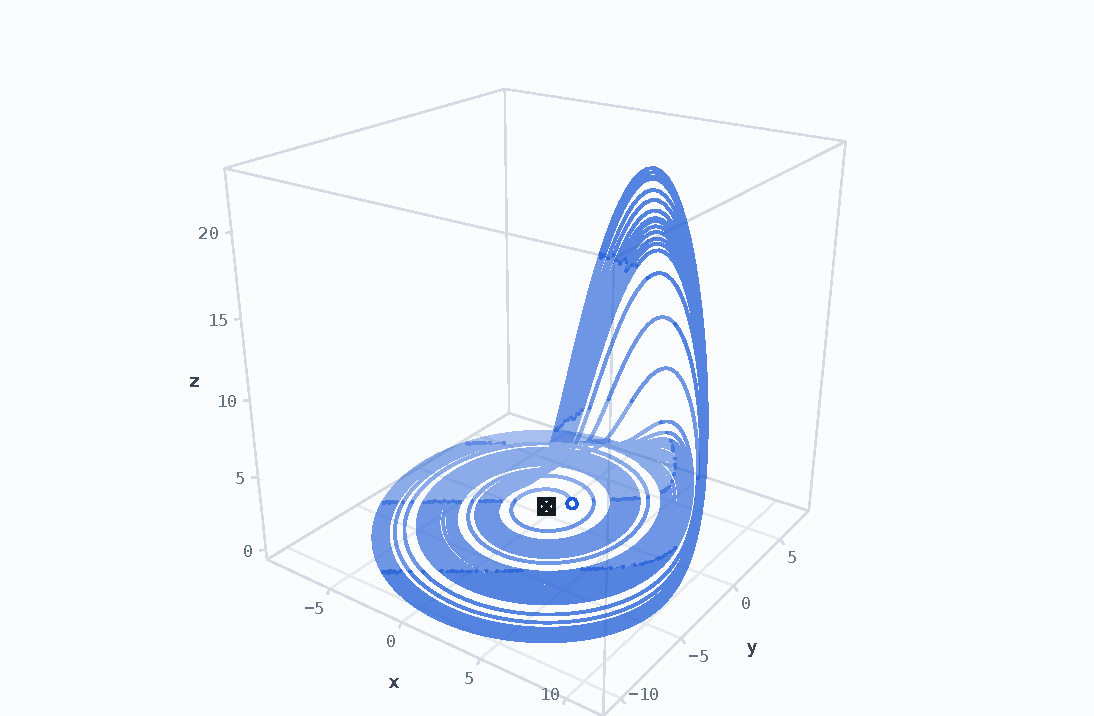
\includegraphics[width=\textwidth]{rossler-3d.pdf}
  \end{minipage}\hfill
  \begin{minipage}[t]{0.5\textwidth}\centering
    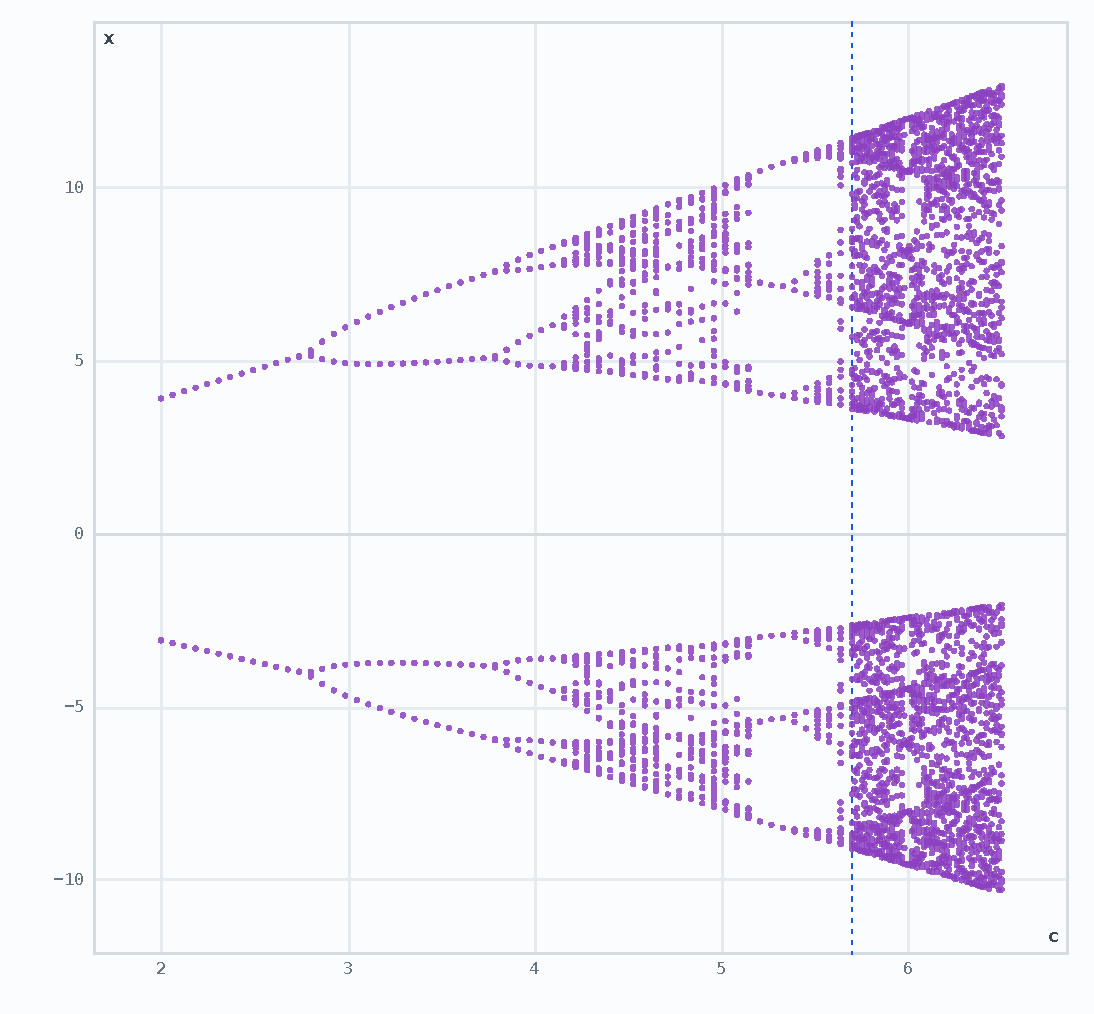
\includegraphics[width=\textwidth]{rossler-sweep.pdf}
  \end{minipage}
  \caption{Rössler system at $a=b=0.2$. Left: the chaotic attractor at $c=5.7$ in the 3D view. Right: \ui{Sweep max/min} in $c$, showing the local maxima and minima of $x$ and the period-doubling route to chaos.}
  \label{fig:rossler}
\end{figure}

Load \ui{Rössler system} \cite{rossler1976} and press \key{2}. Drag to rotate the attractor, scroll to zoom, or press \ui{Spin}. The axes are chosen in the toolbar, and any of them can be time.

\begin{tryit}
\begin{enumerate}
  \item In the Bifurcation view choose $c$ and press \ui{Sweep max/min} (Figure~\ref{fig:rossler}, right). The number of parameter values is set by \ui{Sweep samples} in the Numerics tab.
  \item For a continuation version, set $c=2.5$, integrate onto the stable cycle and press \ui{Limit cycle}. Period doublings are found at $c\approx 2.8324$, $3.8374$, $4.1242$ and $4.1870$. Pressing \ui{Double} at each in turn follows the cascade.
  \item \ui{Follow} on a PD point traces its curve in $(c,a)$.
\end{enumerate}
\end{tryit}

% ==================================================================
\section{Tutorial 5: maps}\label{sec:maps}

\begin{figure}[t]
  \centering
  \begin{minipage}[t]{0.47\textwidth}\centering
    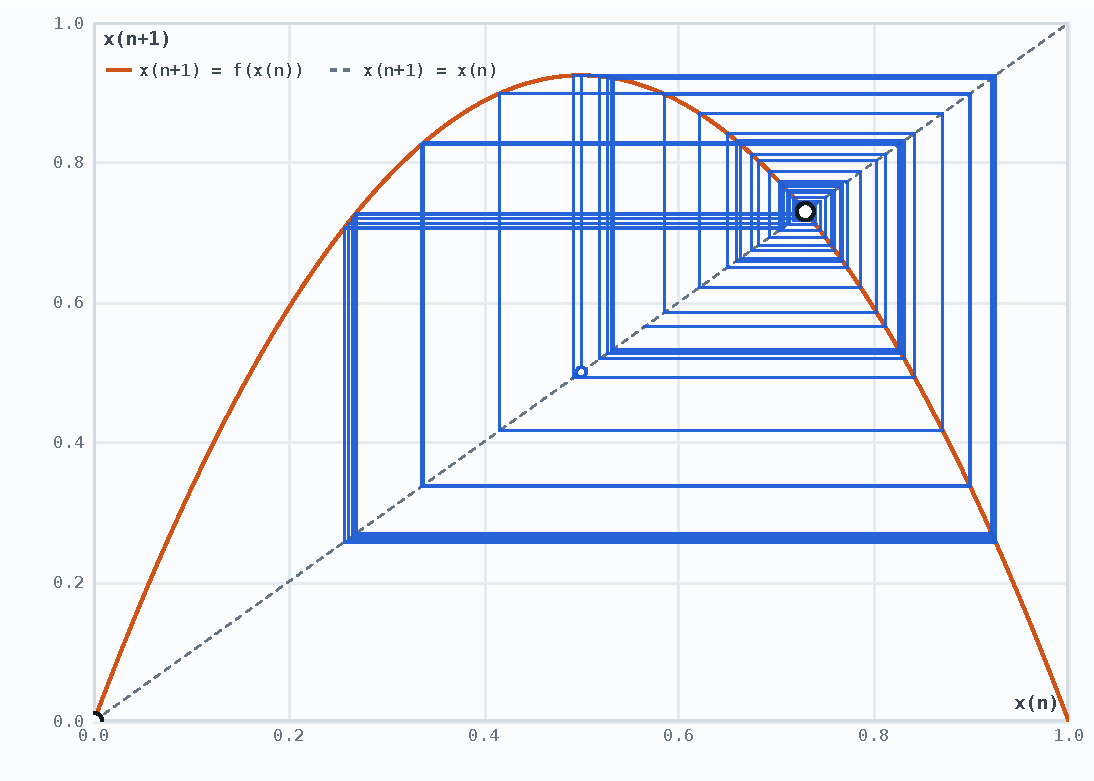
\includegraphics[width=\textwidth]{logistic-cobweb.pdf}
  \end{minipage}\hfill
  \begin{minipage}[t]{0.5\textwidth}\centering
    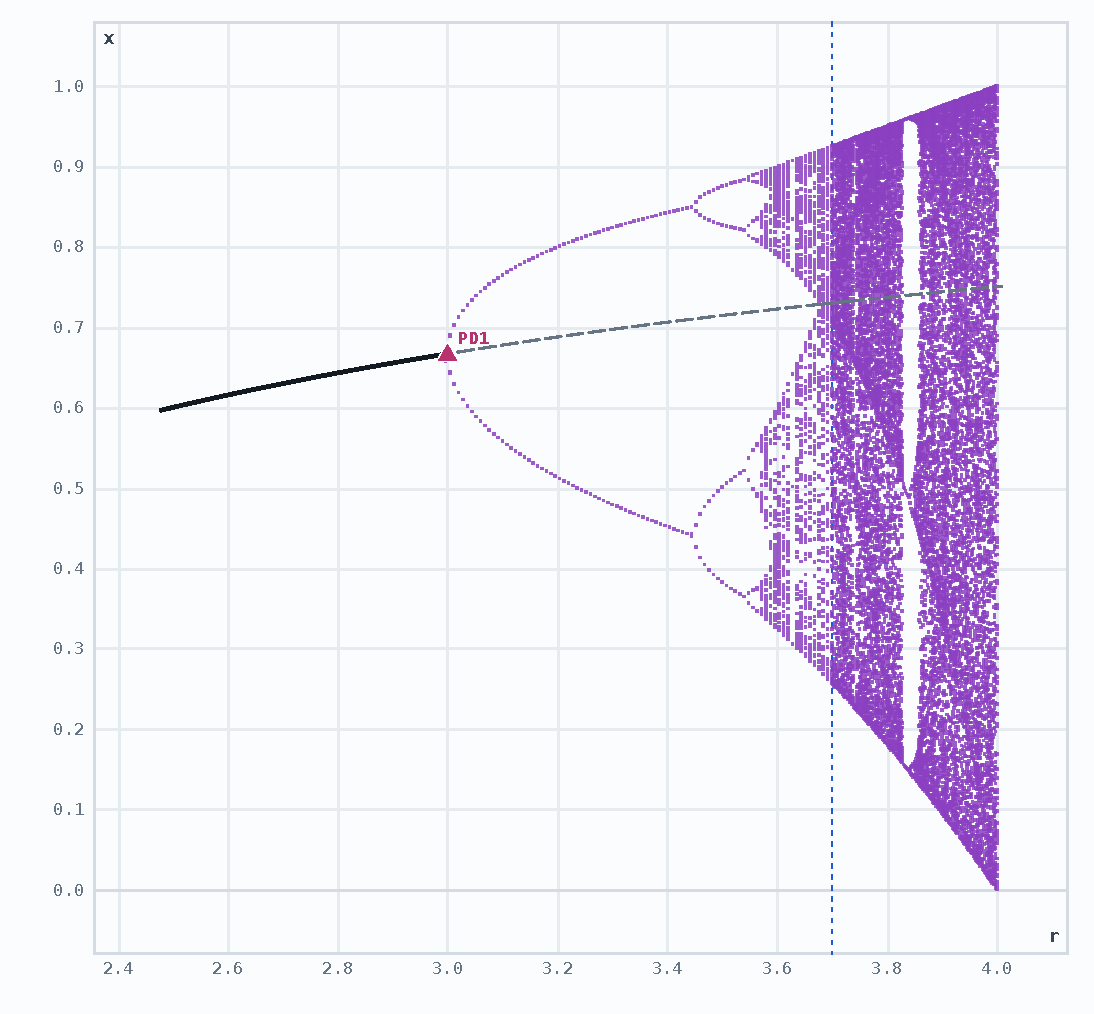
\includegraphics[width=\textwidth]{logistic-orbit.pdf}
  \end{minipage}
  \caption{Logistic map $x\mapsto rx(1-x)$. Left: cobweb diagram at $r=3.7$. Right: orbit diagram from \ui{Sweep max/min} (purple dots), with the continued fixed point and its period doubling PD1 at $r=3$.}
  \label{fig:logistic}
\end{figure}

A model is a map when its equations are written \texttt{x(t+1)=\ldots}. Trajectories are then drawn as points, and for a one-variable map the phase plane becomes a cobweb diagram (Figure~\ref{fig:logistic}). For maps, \ui{Sweep max/min} keeps up to 250 iterates after the transient, which gives the familiar orbit diagram. Continuation finds folds, period doublings and Neimark--Sacker points of fixed points. The \ui{Hénon map} example shows a fold at $a\approx-0.1225$ and a PD at $a\approx0.3675$, and the \ui{Delayed logistic map} an NS bifurcation at $a=2$.

% ==================================================================
\section{Tutorial 6: noise and random switching}\label{sec:stoch}

\begin{figure}[t]
  \centering
  \begin{minipage}[t]{0.48\textwidth}\centering
    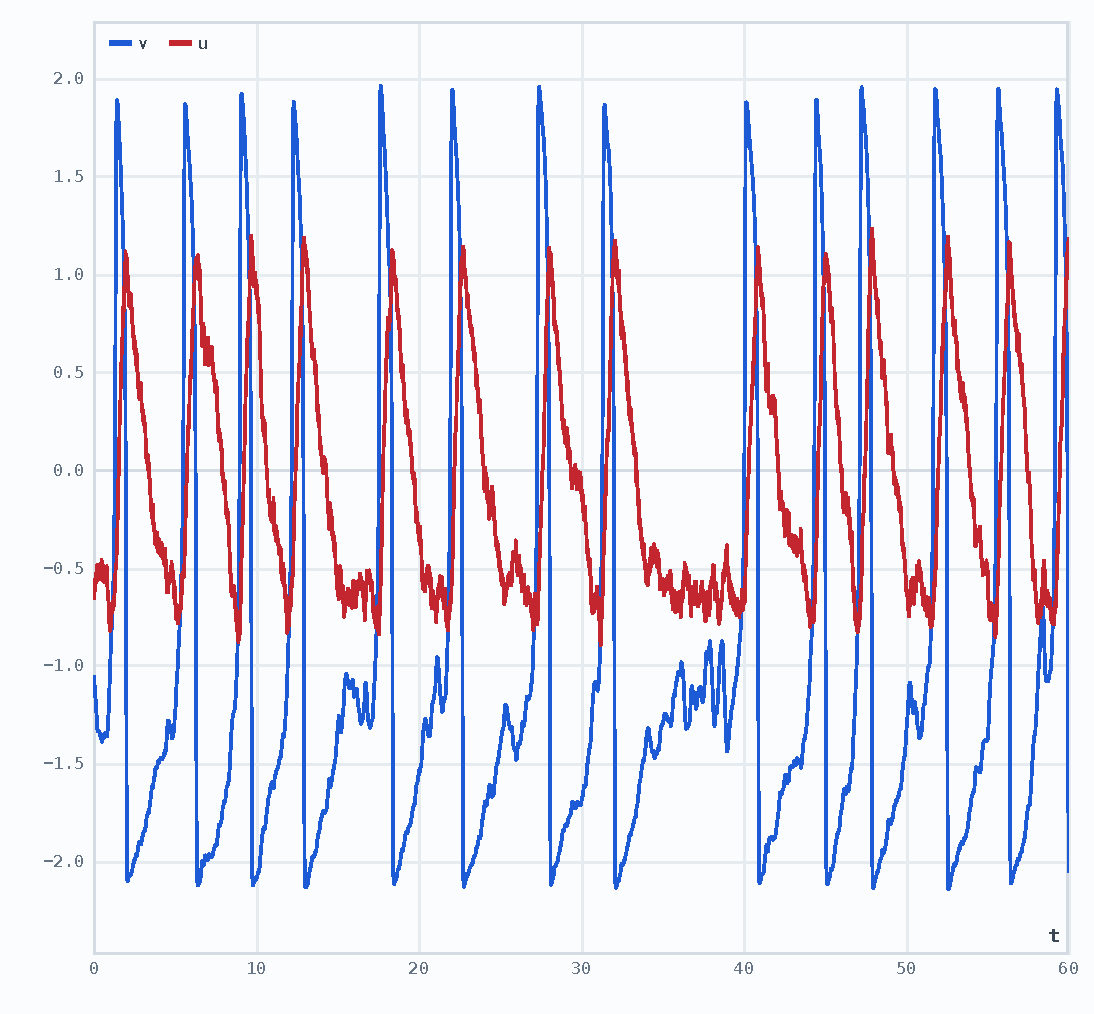
\includegraphics[width=\textwidth]{nfhn-timecourse.pdf}
  \end{minipage}\hfill
  \begin{minipage}[t]{0.48\textwidth}\centering
    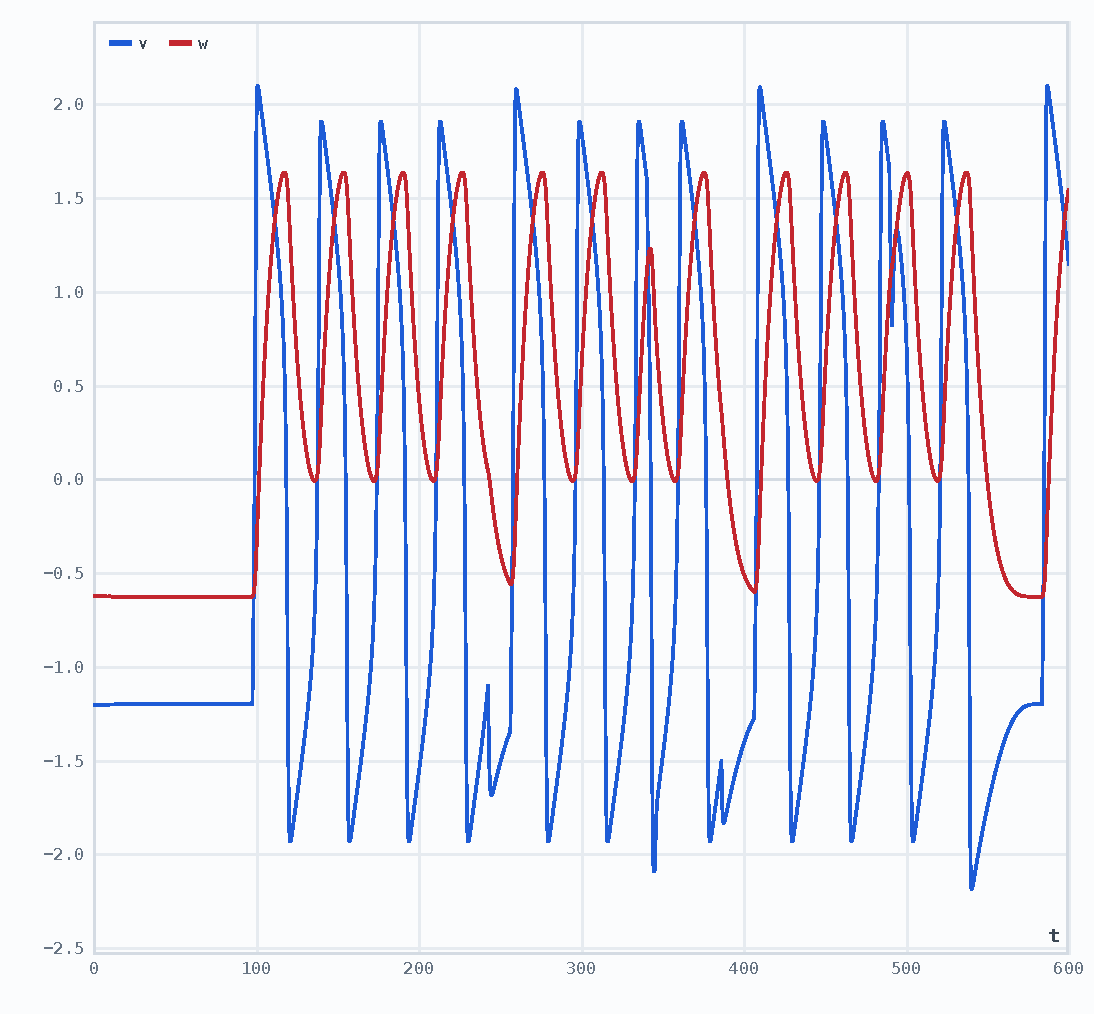
\includegraphics[width=\textwidth]{tfhn-timecourse.pdf}
  \end{minipage}
  \caption{Left: excitable FitzHugh--Nagumo driven by white noise; noise triggers irregular spikes. Right: FitzHugh--Nagumo whose input is a two-state Markov variable, so oscillation switches on and off at random.}
  \label{fig:stoch}
\end{figure}

\paragraph{Wiener noise.} Declaring \texttt{wiener w} makes \texttt{w} a white-noise source. The equations are integrated by Euler--Maruyama with step \texttt{dt}, and over each step \texttt{w} is $N(0,1)/\sqrt{dt}$, exactly as in \XPP{}. In \ui{Noisy FitzHugh--Nagumo} the rest state is stable, and noise of amplitude \texttt{sig} kicks the system over threshold (Figure~\ref{fig:stoch}, left). Drag \texttt{sig} to change the firing rate.

\paragraph{Markov variables.} \ui{Telegraph-driven FitzHugh--Nagumo} declares
\begin{lstlisting}
markov s 2
{0} {kon}
{koff} {0}
\end{lstlisting}
a variable that jumps $0\to1$ at rate \texttt{kon} and $1\to0$ at rate \texttt{koff}. Rates may depend on the state variables. The input \texttt{i0+di*s} switches the cell between rest and oscillation (Figure~\ref{fig:stoch}, right).

\paragraph{Seeds.} Each stochastic run uses a new random seed, which is reported in the status line. Enter a number in \ui{Noise seed} (Numerics tab), or write \texttt{@ seed=7}, to repeat the same noise path, for instance to compare parameter values. Equilibria, nullclines and continuation always use the noise-free system, with Markov states held at the values in the Initial tab.

% ==================================================================
\section{Tutorial 7: stiff systems}\label{sec:stiff}

The \ui{Stiff van der Pol} example has $\mu=1000$: relaxation oscillations whose slow and fast time scales differ by a factor of about $10^6$. With \texttt{@ meth=stiff} the Rosenbrock 2(3) solver integrates a period ($T\approx1614.4$) in a few thousand steps, where an explicit method needs hundreds of thousands. When the stiff method is selected, periodic-orbit continuation also uses it for its shooting segments, so the period can be continued down in $\mu$.

% ==================================================================
\section{Tutorial 8: arrays and Volterra equations}\label{sec:volterra}

\begin{figure}[t]
  \centering
  \begin{minipage}[t]{0.48\textwidth}\centering
    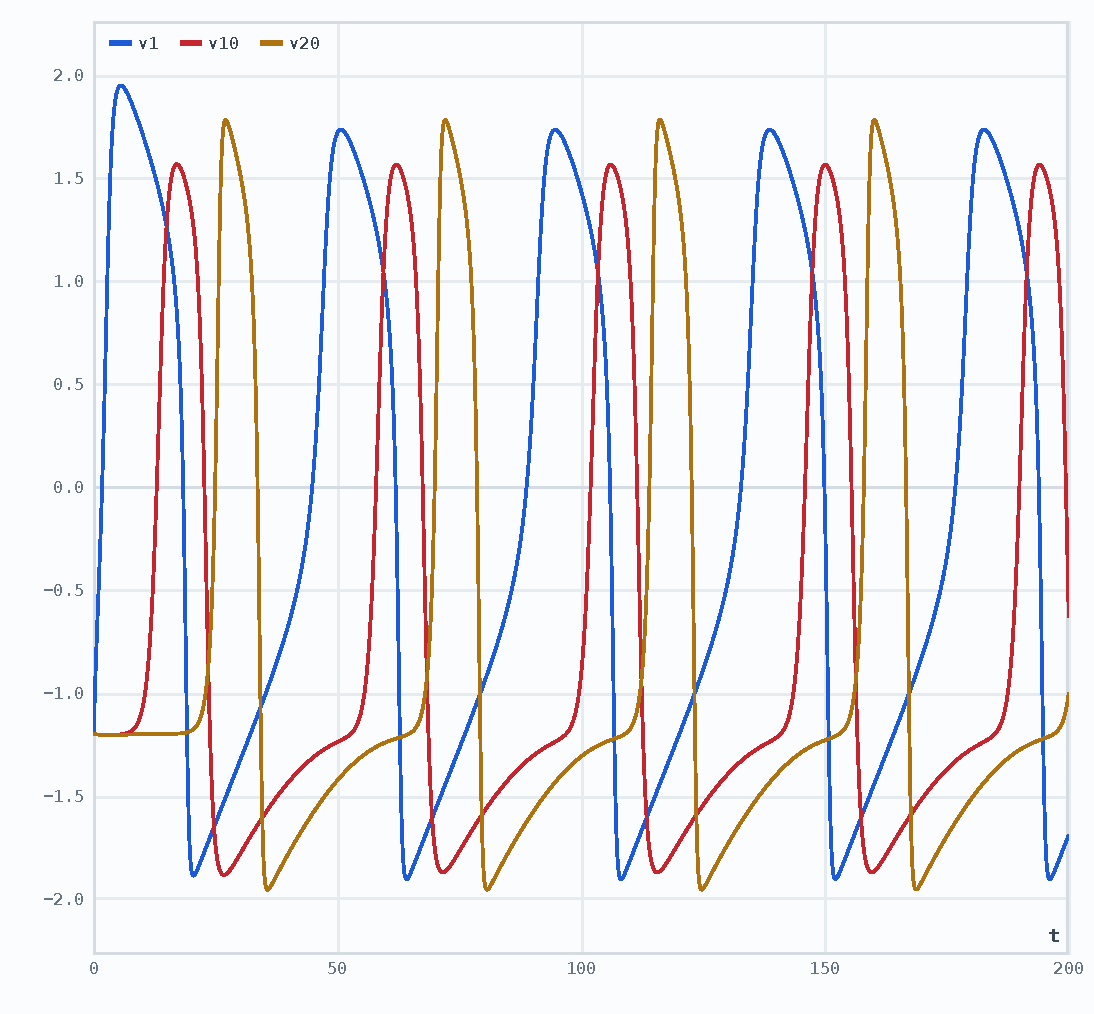
\includegraphics[width=\textwidth]{chain-timecourse.pdf}
  \end{minipage}\hfill
  \begin{minipage}[t]{0.48\textwidth}\centering
    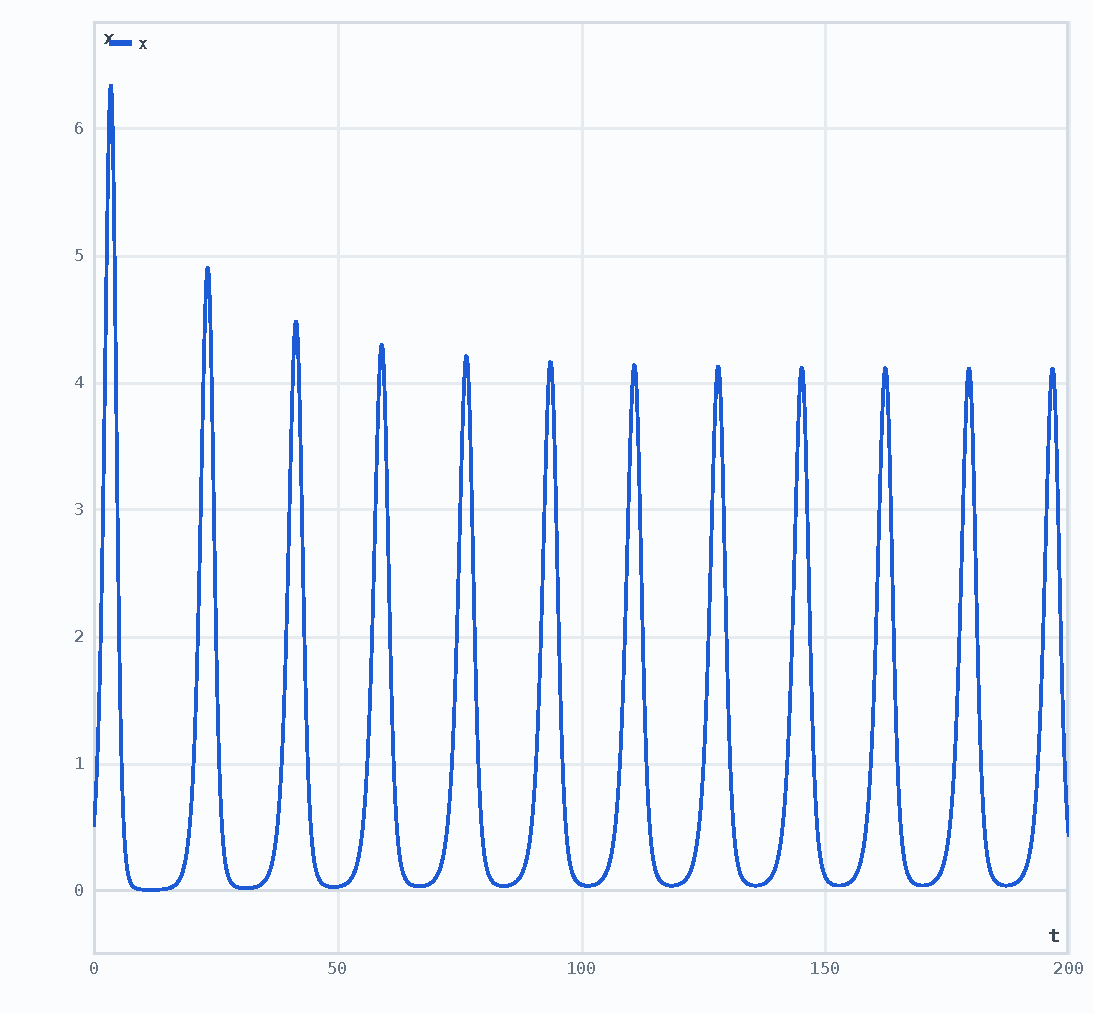
\includegraphics[width=\textwidth]{dlogv-timecourse.pdf}
  \end{minipage}
  \caption{Left: a chain of 20 FitzHugh--Nagumo cells written with arrays. Spikes start at cell 1 and arrive later at cells 10 and 20. Right: logistic growth with a gamma-distributed delay, written as a Volterra convolution. At $r\tau=2.5$ the equilibrium is unstable and the population oscillates.}
  \label{fig:arrays}
\end{figure}

\paragraph{Arrays.} \XPP{}'s arrays are a text macro. The \ui{Chain of 20 FitzHugh--Nagumo cells} example is written as
\begin{lstlisting}
%[1..20]
v[j]'=v[j]-v[j]^3/3-w[j]+i1*heav(1.5-[j])+d*(v[j+1]-2*v[j]+v[j-1])
%
w[1..20]'=eps*(v[j]+a-b*w[j])
v0=v1
v21=v20
init v[1..20]=-1.2
init w[1..20]=-0.62
\end{lstlisting}
The block between \texttt{\%[1..20]} and \texttt{\%} is repeated for $j=1,\ldots,20$. Every \texttt{[expr]} is replaced by its integer value, so \texttt{v[j-1]} becomes \texttt{v3} when $j=4$, and \texttt{[j]} on its own becomes the number~$j$. A single line containing \texttt{[1..20]} is repeated the same way. The load message reports how many lines the file expanded to. The expanded model is an ordinary 40-dimensional system, so its equilibria, eigenvalues (computed by the QR algorithm) and continuation all work as usual. In Figure~\ref{fig:arrays} (left) the time course shows $v_1$, $v_{10}$ and $v_{20}$; choose them with the chips in the inspector.

\paragraph{Volterra integrals.} \XS{} supports \XPP{}'s integral terms:
\begin{itemize}
  \item \texttt{int\{K(t,t',x)\}} $=\int_0^t K(t,t',x(t'))\,dt'$, where the variables inside are evaluated at $t'$;
  \item \texttt{int\{K\#x\}} $=\int_0^t K(t-t')\,x(t')\,dt'$, a convolution with the kernel written as a function of $t$;
  \item \texttt{int[mu]\{\ldots\}} adds the weakly singular factor $(t-t')^{-\mu}$, $0\le\mu<1$;
  \item \texttt{u(t)=\ldots} or \texttt{volterra u=\ldots} defines a variable by an integral equation.
\end{itemize}
The \ui{Logistic growth with distributed delay} example is
\begin{lstlisting}
x'=r*x*(1-int{t*exp(-t/tau)/tau^2#x})
par r=1,tau=2.5
@ total=200,dt=0.05,vmaxpts=1000
\end{lstlisting}
The kernel $K(s)=s\,e^{-s/\tau}/\tau^2$ has mean delay $2\tau$. Linearising about $x=1$ gives $\lambda(1+\lambda\tau)^2+r=0$, so the equilibrium loses stability in a Hopf bifurcation at $r\tau=2$. Sweeping $\tau$ with \ui{Sweep max/min} shows the oscillation appear.

Integro-differential equations are solved by a fixed-step method: the trapezoid rule for the differential part and product-trapezoid quadrature \cite{linz1985} for the integrals. The quadrature weights are exact for the $(t-t')^{-\mu}$ factor, and the implicit terms are found by fixed-point iteration. The error falls as $dt^2$, or as $dt^{2-\mu}$ with a singular kernel. The method reproduces $u(t)=e^t$ for $u=1+\int_0^t u$, and the solution $e^{\pi t}\operatorname{erfc}(\sqrt{\pi t})$ of the Abel equation \texttt{u(t)=1-int[.5]\{1\#u\}}. It also agrees with the equivalent three-variable ODE for the gamma kernel. Only the last \texttt{vmaxpts} steps are remembered (default 4000). Because the state of such a system is its whole history, equilibria, nullclines and continuation are switched off for these models. Trajectories and sweeps work normally.

\paragraph{Periodic variables and tables.} Two further \XPP{} features are worth knowing:
\begin{itemize}
  \item \texttt{@ fold=th} keeps an angle in $[0,2\pi)$ (or $[0,\texttt{tor\_per})$). Plots break the trajectory where it wraps, and continuation measures distances modulo the period; see the \ui{Driven pendulum} example.
  \item Tables (\ui{Phase oscillators with a tabulated H}) are interpolated linearly. They can be sampled from an expression or read from a data file.
\end{itemize}

% ==================================================================
\section{Tutorial 9: delay equations}\label{sec:dde}

\begin{figure}[t]
  \centering
  \begin{minipage}[t]{0.48\textwidth}\centering
    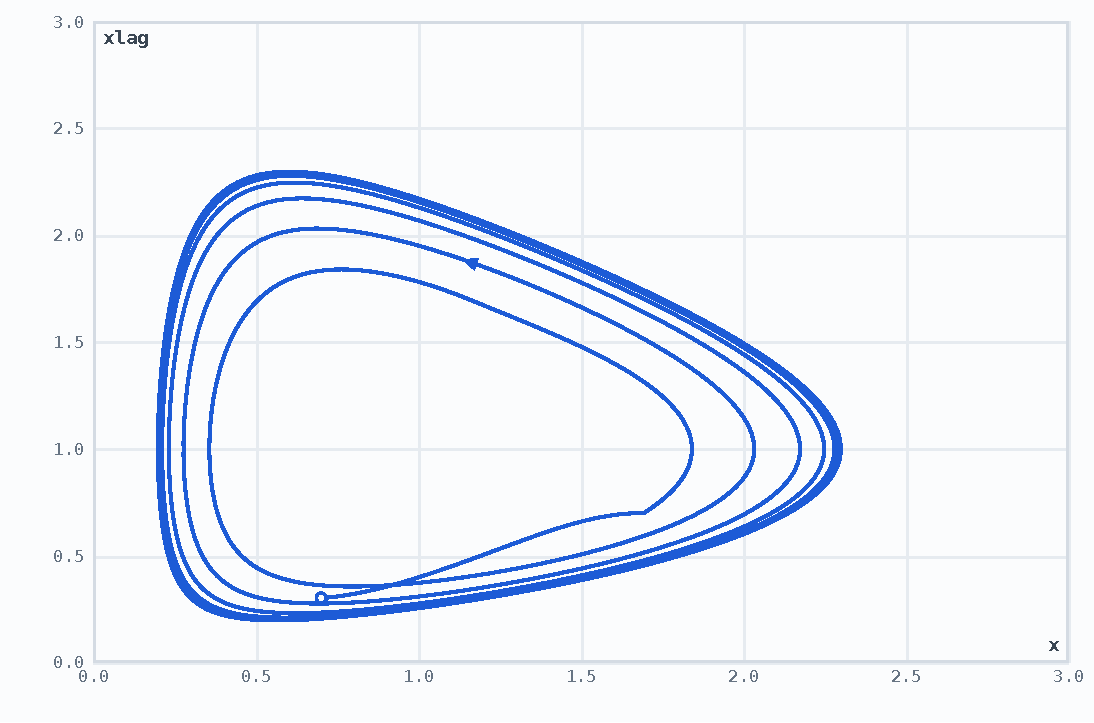
\includegraphics[width=\textwidth]{hutch-pp.pdf}
  \end{minipage}\hfill
  \begin{minipage}[t]{0.48\textwidth}\centering
    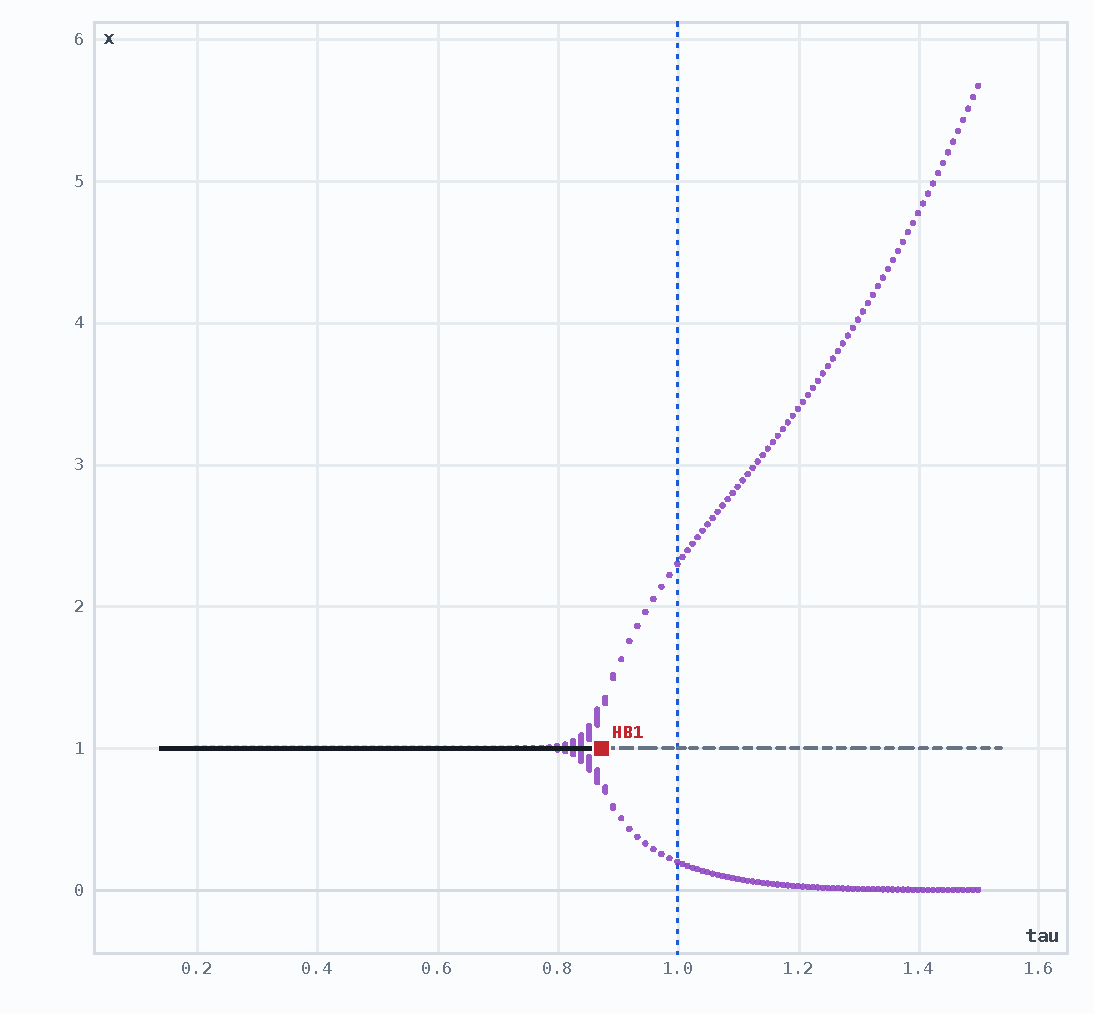
\includegraphics[width=\textwidth]{hutch-bif.pdf}
  \end{minipage}
  \caption{Hutchinson's delayed logistic equation with $r=1.8$. Left: $x(t-\tau)$ against $x(t)$ for $\tau=1$, starting from the history $0.5+0.2\cos 3t$ and settling onto a periodic orbit. Right: bifurcation diagram in $\tau$. The equilibrium $x=1$ (black) loses stability at the Hopf point HB1, $\tau\approx0.874$, close to the exact value $\pi/(2r)=0.873$. The purple dots, from \ui{Sweep max/min}, show the oscillation that grows from it.}
  \label{fig:hutch}
\end{figure}

A delay-differential equation uses past values of its variables. In \XS{}, as in \XPP{}, \texttt{delay(x,tau)} stands for $x(t-\tau)$, where \texttt{x} must be a variable with an equation and \texttt{tau} is any expression; it may depend on the state. Load \ui{Delayed logistic equation}, Hutchinson's model \cite{hutchinson1948}:
\begin{lstlisting}
x'=r*x*(1-delay(x,tau))
aux xlag=delay(x,tau)
par r=1.8,tau=1
x(0)=0.5+0.2*cos(3*t)
\end{lstlisting}

\paragraph{History.} A delay equation needs its state on a whole interval $[-\tau,0]$, not only at $t=0$. Writing \texttt{x(0)} as a formula in \texttt{t} gives that history, and its value at $t=0$ becomes the initial condition. Without a formula, the history is held constant at the initial value. The formulas also appear in the \ui{Initial} tab under \ui{History for t < 0} (Figure~\ref{fig:history}), where they can be changed or cleared. Clicking the phase plane changes only the values at $t=0$. The auxiliary variable \texttt{xlag} makes $x(t-\tau)$ available for plotting, so the phase plane in Figure~\ref{fig:hutch} shows $x(t-\tau)$ against $x(t)$, a common way to draw the attractor of a scalar delay equation.

\begin{figure}[h]
  \centering
  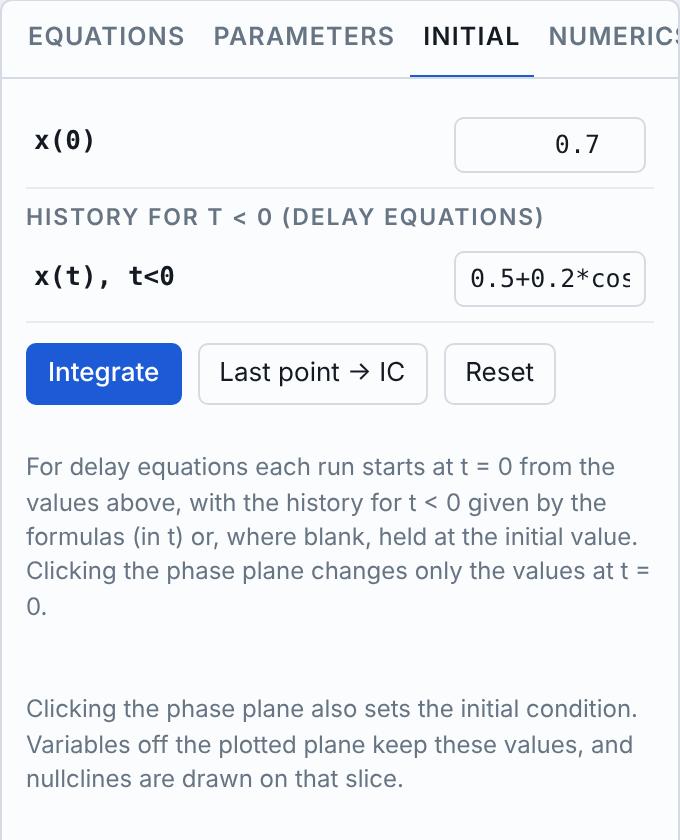
\includegraphics[width=0.5\textwidth]{ui-history.png}
  \caption{The Initial tab for a delay equation: the value at $t=0$ and, below it, the history for $t<0$ as a formula in $t$.}
  \label{fig:history}
\end{figure}

\paragraph{Integration.} Delay equations run forward from $t=0$ with fixed-step fourth-order Runge--Kutta (adaptive methods fall back to it). Every step is stored, and delayed values are found by cubic Hermite interpolation of the stored solution, or from the history when $t-\tau<0$. For $x'=-x(t-1)$ with $x=1$ on $[-1,0]$, whose exact solution is piecewise polynomial, the computed $x(2)$ and $x(3)$ agree with the exact values to rounding error.

\paragraph{Stability and continuation.} Equilibria of a delay equation are those of the system with the delays removed, but their stability is not. It is set by the roots of the characteristic equation
\[
\det\Bigl(\lambda I-A_0-\sum_k B_k\,e^{-\lambda\tau_k}\Bigr)=0,
\]
where $A_0$ and $B_k$ are the derivatives with respect to the current and the delayed values. There are infinitely many roots, but only finitely many lie to the right of any vertical line. \XS{} approximates the rightmost ones by Chebyshev collocation of the solution operator \cite{breda2005} and then polishes them with Newton's method. The equilibrium list then reports, for example, \emph{Unstable, 2 roots with Re $\lambda>0$} and lists the rightmost roots. \ui{Continue equilibria} uses the same roots, so Hopf points are those of the delay equation.

\begin{tryit}
\begin{enumerate}
  \item Load \ui{Delayed logistic equation} and press \key{G}. With $r\tau=1.8>\pi/2$ the solution settles onto a periodic orbit (Figure~\ref{fig:hutch}, left). Change the history formula in the Initial tab and integrate again.
  \item The inspector lists two equilibria. $x=0$ has the single root $\lambda=r$. $x=1$ has a complex pair $\lambda\approx0.097\pm1.63i$ in the right half-plane.
  \item In the Bifurcation view choose \texttt{tau}, a range of $0.2$ to $1.5$ and \ui{Step ds} $0.02$, then press \ui{Continue equilibria}. A Hopf point HB1 is found at $\tau\approx0.874$, against $\pi/(2r)=0.8727$. \ui{Sweep max/min} adds the oscillation amplitude (Figure~\ref{fig:hutch}, right).
  \item Load \ui{Mackey--Glass equation} \cite{mackey1977} (Figure~\ref{fig:mg}). With $\tau=17$ the solution is chaotic; the file uses \texttt{@ trans=300} to drop the transient. Continuation in $\tau$ finds Hopf points at $\tau\approx4.71$ and $20.98$. Linearising by hand gives $\lambda=-0.1-0.4\,e^{-\lambda\tau}$, with Hopf points at $\tau=4.708$ and $20.93$.
\end{enumerate}
\end{tryit}

\begin{figure}[t]
  \centering
  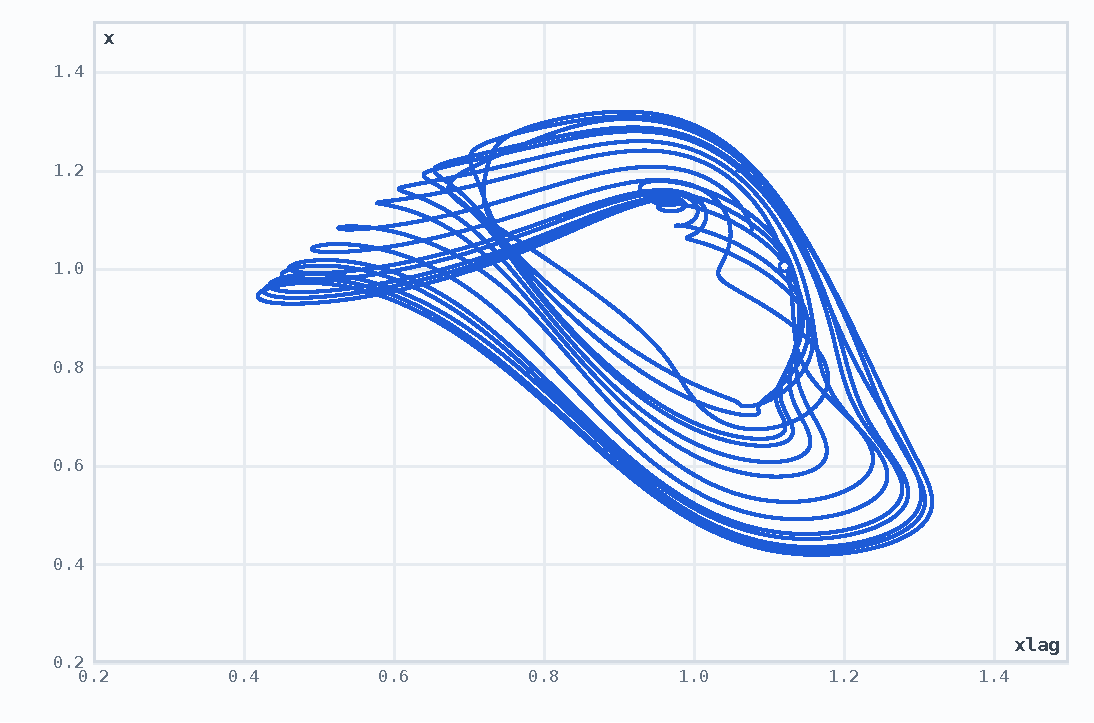
\includegraphics[width=0.5\textwidth]{mg-pp.pdf}
  \caption{The chaotic Mackey--Glass attractor at $\tau=17$, drawn as $x(t)$ against $x(t-\tau)$ after a transient of 300.}
  \label{fig:mg}
\end{figure}

\noindent Periodic-orbit and two-parameter continuation, the direction field and the derivative readout are switched off for delay equations, because the state at time $t$ is a whole function rather than a point.

% ==================================================================
\section{Tutorial 10: events and global flags}\label{sec:flags}

\begin{figure}[t]
  \centering
  \begin{minipage}[t]{0.48\textwidth}\centering
    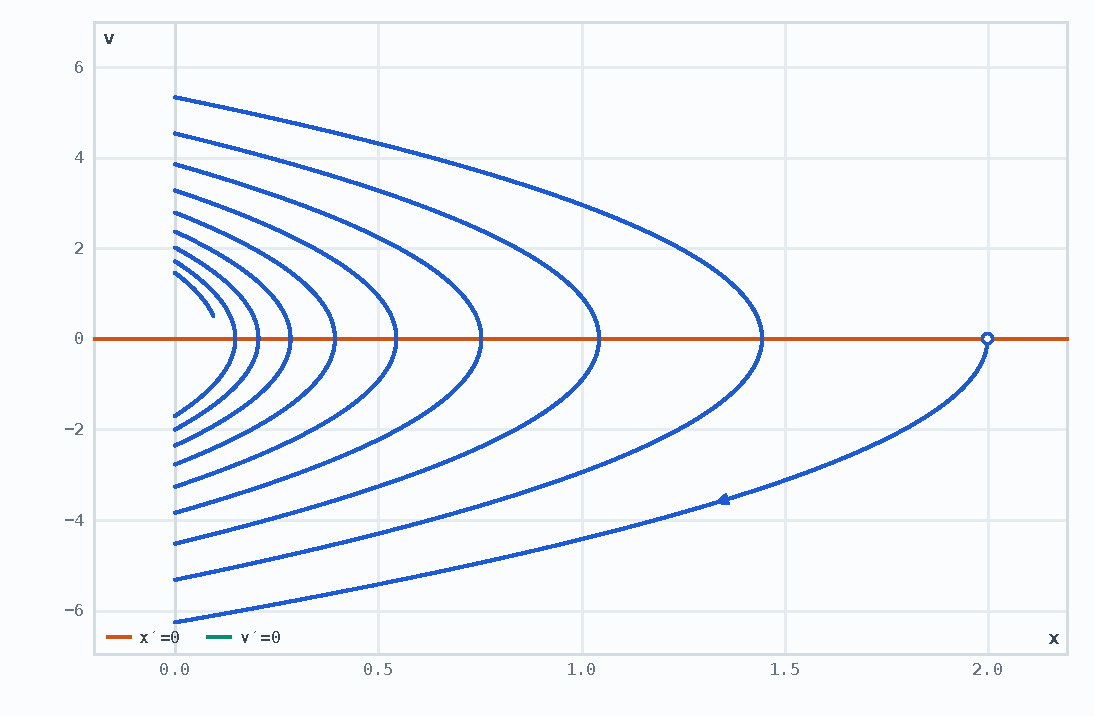
\includegraphics[width=\textwidth]{ball-pp.pdf}
  \end{minipage}\hfill
  \begin{minipage}[t]{0.48\textwidth}\centering
    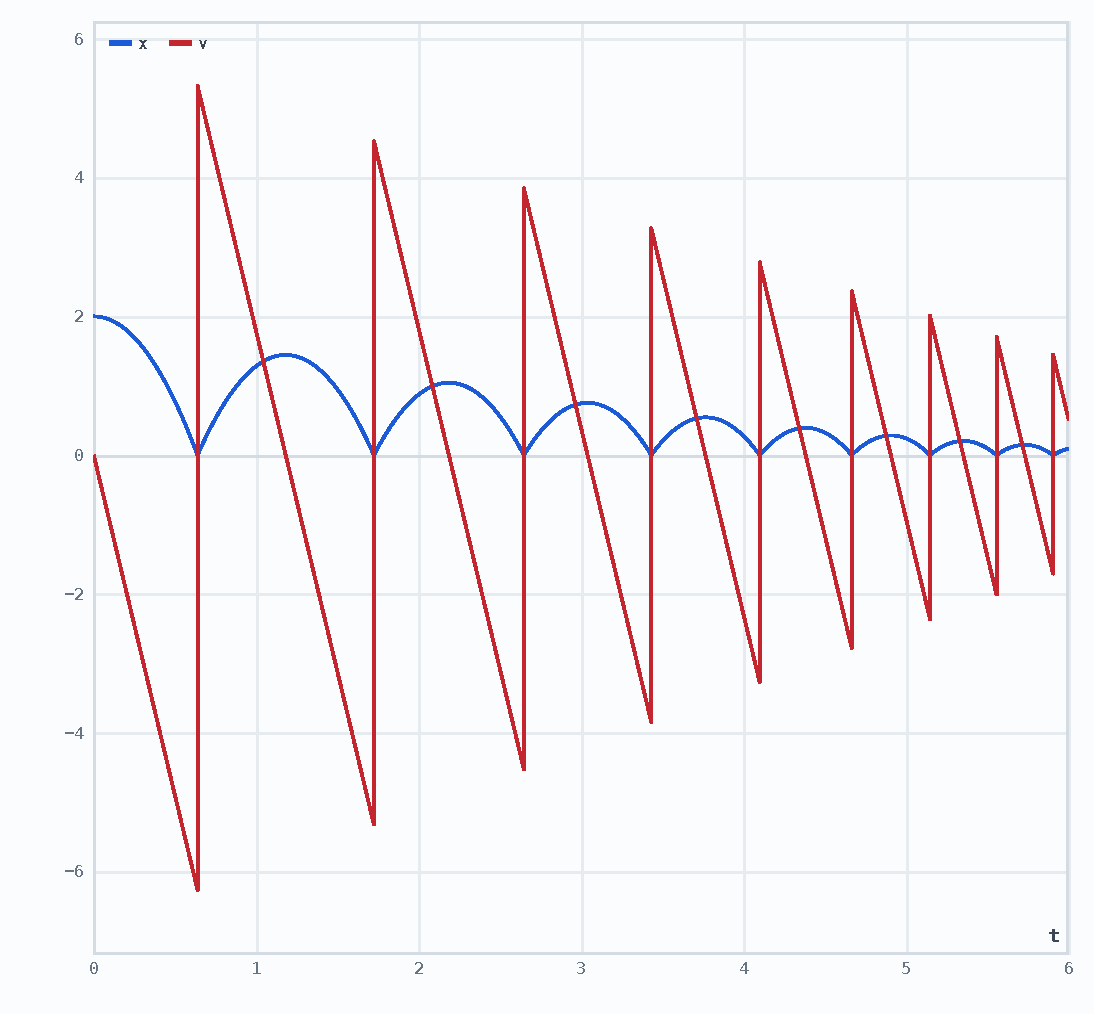
\includegraphics[width=\textwidth]{ball-tc.pdf}
  \end{minipage}
  \caption{The bouncing ball. Left: velocity against height. Each parabola is one flight, and the line breaks at each event instead of joining the points before and after it. Right: height $x$ (blue) and velocity $v$ (red) against time, with the jump in $v$ at each bounce.}
  \label{fig:ball}
\end{figure}

Many models change discontinuously when a threshold is reached: a neuron fires and resets, a ball bounces, a switch flips. \XPP{} describes such events with \emph{global flags},
\begin{lstlisting}
global sign condition {name1=expr1;name2=expr2;...}
\end{lstlisting}
The assignments are made when \texttt{condition} crosses zero from negative to positive (\texttt{sign}$=1$), from positive to negative ($-1$), or in either direction (0). All the right-hand sides are evaluated first, then all the assignments are made together. The names may be state or Markov variables, and \texttt{arret=1} stops the integration.

\paragraph{How events are located.} After every step \XS{} checks each condition. If one has crossed zero in its direction, the crossing time is found on the cubic Hermite interpolant of that step, by regula falsi on the condition. The point just before the event and the point just after the assignments are both stored, at the same time, and integration continues from there. This works with every integrator, including the adaptive and stiff ones, and with maps, where the assignments are applied to the new iterate.

\begin{tryit}
\begin{enumerate}
  \item Load \ui{Bouncing ball}:
\begin{lstlisting}
x'=v
v'=-g
global -1 x {x=0;v=-e*v}
\end{lstlisting}
  Press \key{G}. The status line reports the number of events. The first two bounces occur at $t=\sqrt{2x_0/g}=0.6386$ and $t=0.6386\,(1+2e)=1.7242$, and the computed times agree to six decimal places. Each flight is a parabola in the phase plane (Figure~\ref{fig:ball}). Lower the restitution $e$ with its slider and watch the bounces die away faster.
  \item Load \ui{Integrate-and-fire neuron}:
\begin{lstlisting}
v'=(-v+i-w)/tau
w'=-w/tauw
global 1 v-1 {v=0;w=w+b}
\end{lstlisting}
  Each time $v$ reaches threshold it is reset and the adaptation variable $w$ is kicked up, so the firing rate slows until it settles (Figure~\ref{fig:lif}). With $b=0$ the interspike interval is $\tau\ln\bigl(i/(i-1)\bigr)$, and the computed value agrees to six or more digits.
  \item Add \texttt{global 1 t-50 \{arret=1\}} to a model to stop every run at $t=50$.
\end{enumerate}
\end{tryit}

\begin{figure}[t]
  \centering
  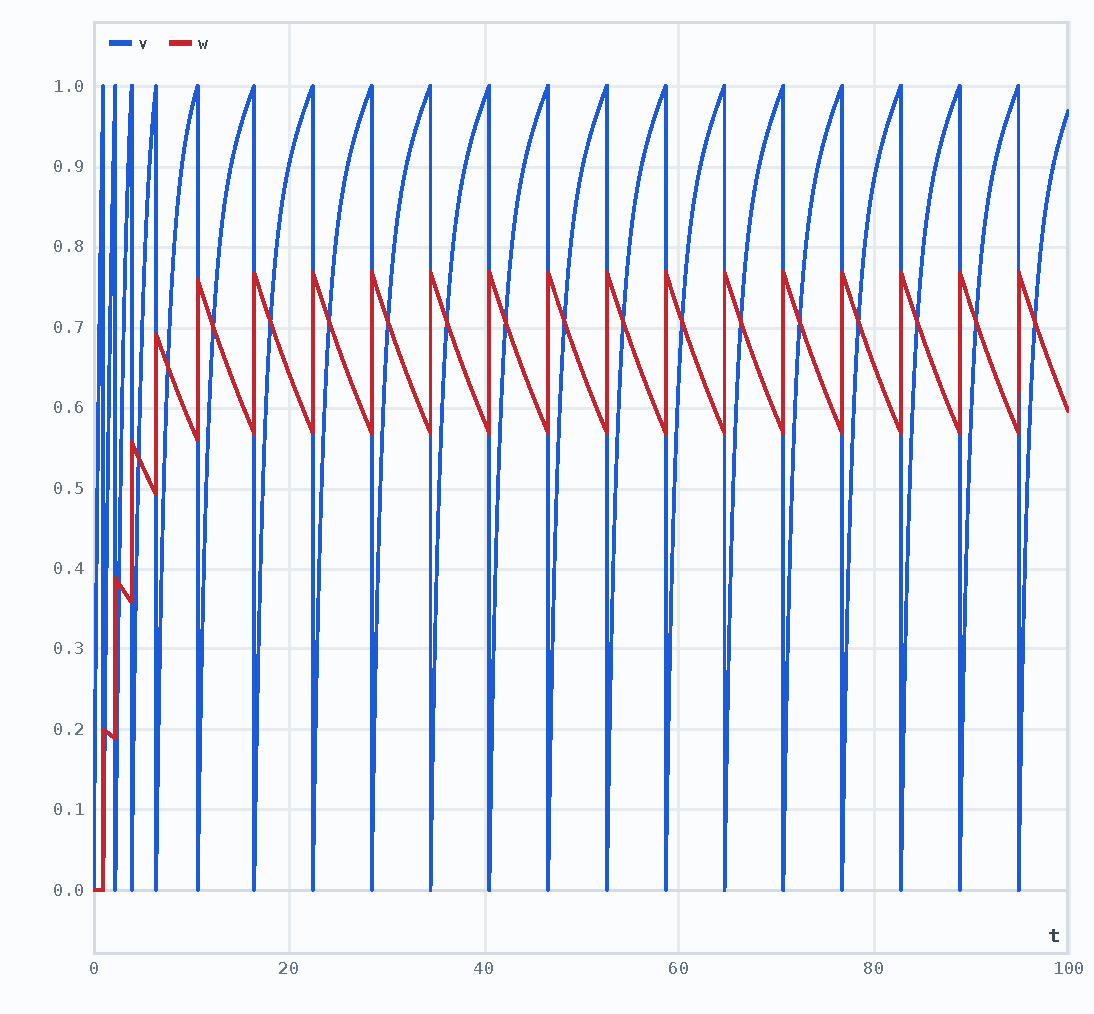
\includegraphics[width=0.55\textwidth]{lif-tc.pdf}
  \caption{Integrate-and-fire neuron with adaptation: $v$ (blue) is reset to 0 at each threshold crossing, while the adaptation current $w$ (red) builds up and lengthens the interspike interval.}
  \label{fig:lif}
\end{figure}

\noindent Equilibria, nullclines and equilibrium continuation ignore flags. Periodic-orbit continuation is switched off for models with flags; use \ui{Sweep max/min} for the long-term behaviour instead.

% ==================================================================
\section{Numerical settings}\label{sec:numerics}

\begin{figure}[t]
  \centering
  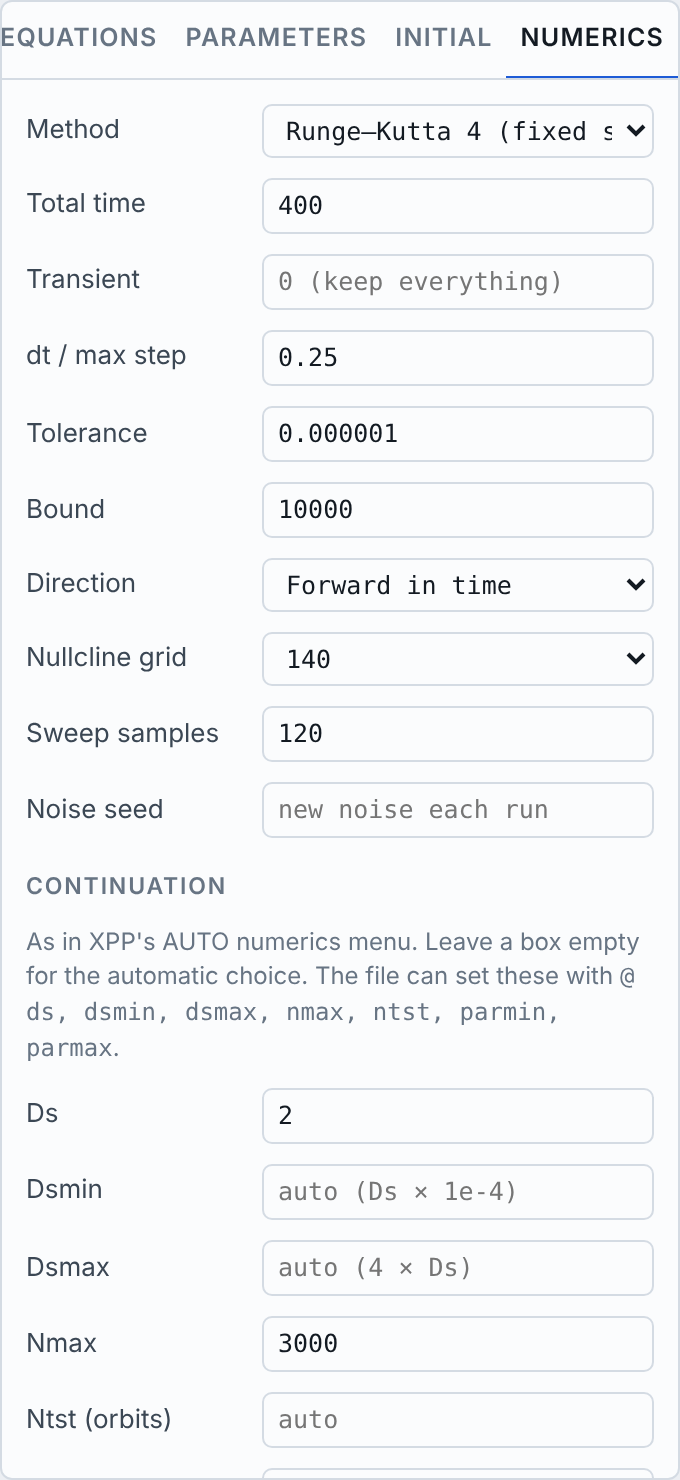
\includegraphics[width=0.42\textwidth]{ui-numerics.png}
  \caption{The Numerics tab: integration settings at the top, continuation settings below.}
  \label{fig:numerics}
\end{figure}

The \ui{Numerics} tab (Figure~\ref{fig:numerics}) collects the integration and continuation parameters. Changes to the integration settings rerun every trajectory on screen.

\paragraph{Integration.}
\begin{description}[font=\sffamily\bfseries]
  \item[Method] As in Section~\ref{sec:language}.
  \item[Total time] The duration of each run; for maps, the number of iterations.
  \item[Transient] As in \XPP{}, the run still lasts the total time, but only $t\ge$ the transient is kept (\texttt{@ trans=}). Use it to look at attractors without the approach to them. Manifolds and the single periods loaded from continuation are never cut.
  \item[dt] The step for fixed-step methods, and the largest step for adaptive ones.
  \item[Tolerance] Applies to the adaptive methods.
  \item[Bound] Integration stops when any variable exceeds this value.
  \item[Direction] Forward or backward in time.
  \item[Nullcline grid] Sets the resolution of the nullclines.
  \item[Sweep samples] Sets the number of parameter values in \ui{Sweep max/min}.
\end{description}

\paragraph{Continuation.} These settings correspond to the entries of \XPP{}'s \textsf{AUTO} numerics window and can be set in the file with \texttt{@ ds, dsmin, dsmax, nmax, ntst, parmin, parmax}. Leave a box empty to use the automatic choice.
\begin{center}\small
\begin{tabularx}{0.95\textwidth}{@{}lX@{}}
\toprule
Setting & Effect\\
\midrule
Ds & initial arclength step for equilibrium branches (same as \ui{Step ds})\\
Dsmin, Dsmax & smallest and largest steps; a branch stops if the step falls below Dsmin\\
Nmax & maximum number of points in each direction of an equilibrium branch\\
Ntst (orbits) & number of shooting intervals per periodic orbit (automatic: 20 for up to 3 variables, 14 up to 5, otherwise 10)\\
Ds, Dsmax, Nmax (orbits) & the same for periodic-orbit branches and curves of cycles\\
Nmax (2-par), Nmax (2-par cycles) & point limits for two-parameter curves\\
\bottomrule
\end{tabularx}
\end{center}
If a branch stops early, the status line says why: for example, it reached the point limit, the corrector stopped converging, the orbit shrank onto a Hopf point, or the period grew without bound (a homoclinic orbit is near). If it stopped because of a step-size or point limit, adjust the corresponding setting and run it again.

% ==================================================================
\section{Saving and exporting results}\label{sec:export}

\begin{description}[font=\sffamily\bfseries]
  \item[Export SVG] Saves the current view as a vector figure with light-theme colours, ready for a paper or for editing in Inkscape or Illustrator. All the plots in this document were made this way.
  \item[Export CSV] Available in the Bifurcation and Two-parameter views.
  \begin{itemize}
    \item The bifurcation table has one row per computed point, with these columns: curve, kind (equilibrium, periodic orbit, sweep or special), label (HB1, LPC2, \ldots), parameter name and value, stability, number of unstable directions, period, the state, and the maximum and minimum of each variable along an orbit.
    \item The two-parameter table has the two parameter values, the period where relevant, the state, and labelled rows for codimension-two points. Hopf curves also get columns for $\ell_1$ and for criticality (subcritical, supercritical or neutral saddle).
    \item In the bifurcation table, special rows for Hopf points give $\ell_1$, and the stability column says subcritical or supercritical.
  \end{itemize}
  \item[Copy CSV] In the trajectory list, copies the current trajectory (time, variables and auxiliaries) to the clipboard.
  \item[Copy text] Copies the \texttt{.ode} file, including any edits, so that it can be saved or used in \XPP{}.
\end{description}

\subsection*{Writing the current state into the file}\label{sec:writestate}
After exploring a model you will often want to keep the parameter values and settings you have arrived at. \ui{Write state}, in the Equations tab, writes them into the \texttt{.ode} text, much as \XPP{} does when it saves a file:
\begin{itemize}
  \item parameter values and initial conditions are changed where they are defined, in the \texttt{par}, \texttt{init} and \texttt{x(0)=} lines, as are slider ranges in \texttt{\#@range} lines and history formulas of delay equations;
  \item the integration settings (method, total time, step, transient, tolerance, bound, random seed), the plot axes and window, and the continuation settings are collected in \texttt{@} lines just before \texttt{done}.
\end{itemize}
For example, after setting $i=150$ and a transient of 100 in the Morris--Lecar example, the end of the file reads
\begin{lstlisting}
param i=150,c=20
...
# Settings written by XPP Studio, 2026-10-20 10:30
@ meth=rungekutta, total=400, dt=0.25, trans=100, bound=10000
@ xp=v, yp=w, zp=ica, xlo=-75, xhi=45, ylo=-0.1, yhi=0.55
@ ds=2, nmax=3000, parmin=0, parmax=300
done
\end{lstlisting}
Pressing \ui{Write state} again replaces this block rather than adding another, and \ui{Apply} on the result restores exactly the same state. The text is not reloaded, so the trajectories on screen are kept. Use \ui{Copy text}, or your browser's own storage of the editor, to keep the file. Parameters defined through array lines are left as written.

% ==================================================================
\section{Differences from \XPP{}}

\XS{} aims to read the same files and to feel familiar, but it is a reimplementation:
\begin{itemize}
  \item \textbf{Continuation.} It is built in and written from scratch: pseudo-arclength continuation of equilibria, and multiple shooting (rather than \textsf{AUTO}'s orthogonal collocation) for periodic orbits. Results agree with \textsf{AUTO} to plotting accuracy on the examples, but very long or very unstable orbits may need more shooting intervals (Ntst).
  \item \textbf{Delay equations} are integrated with a fixed step only, and periodic orbits of delay equations cannot be continued. \XPP{}'s other delay options, such as \texttt{delshft} and \texttt{ndelay}, are not supported. The \texttt{@ delay} option is accepted but not needed, since all of the history is kept.
  \item \textbf{Global flags} can set state and Markov variables and \texttt{arret}. The XPP output flag \texttt{out\_put} is accepted and ignored.
  \item \textbf{Not supported:} boundary-value problems (\texttt{bdry}), \texttt{special} and \texttt{export} declarations, and \texttt{set} blocks.
  \item \textbf{Two-parameter Hopf curves} are limited to 12 variables, because the bialternate product grows quadratically with dimension.
  \item \textbf{Volterra models} cannot be continued, since their state is infinite-dimensional.
  \item \textbf{Browser files.} Files are opened and saved through the browser. Table data files are kept in the browser's local storage until you press \ui{Forget table files}.
\end{itemize}

% ==================================================================
\section{Credits and licence}

\XS{} is inspired by, and reads the model files of, \XPP{} by G.~Bard Ermentrout (University of Pittsburgh), described in \cite{ermentrout2002}. Its continuation methods follow the ideas of \textsf{AUTO} \cite{doedel2007} by Eusebius Doedel and colleagues, and of \textsf{MatCont} \cite{dhooge2003}. This version (October 2026) was created by Peter Ashwin and Bard Ermentrout in collaboration with Claude Opus 5.5, an AI model made by Anthropic.

\XS{} is free software, released under the GNU General Public License, version~3 or later. The licence text is distributed with the program (\texttt{LICENSE.txt}) and is available at \url{https://www.gnu.org/licenses/gpl-3.0.html}.

% ==================================================================
\begin{thebibliography}{99}\small
\bibitem{ermentrout2002} G.~B. Ermentrout, \emph{Simulating, Analyzing, and Animating Dynamical Systems: A Guide to XPPAUT for Researchers and Students}, SIAM, Philadelphia, 2002.
\bibitem{doedel2007} E.~J. Doedel, A.~R. Champneys, F.~Dercole, T.~F. Fairgrieve, Yu.~A. Kuznetsov, B.~Oldeman, R.~C. Paffenroth, B.~Sandstede, X.~J. Wang and C.~Zhang, \emph{AUTO-07P: Continuation and bifurcation software for ordinary differential equations}, Concordia University, 2007.
\bibitem{dhooge2003} A.~Dhooge, W.~Govaerts and Yu.~A. Kuznetsov, MATCONT: a MATLAB package for numerical bifurcation analysis of ODEs, \emph{ACM Trans.\ Math.\ Software} \textbf{29} (2003) 141--164.
\bibitem{govaerts2000} W.~J.~F. Govaerts, \emph{Numerical Methods for Bifurcations of Dynamical Equilibria}, SIAM, Philadelphia, 2000.
\bibitem{kuznetsov2004} Yu.~A. Kuznetsov, \emph{Elements of Applied Bifurcation Theory}, 3rd edn, Springer, New York, 2004.
\bibitem{keller1977} H.~B. Keller, Numerical solution of bifurcation and nonlinear eigenvalue problems, in \emph{Applications of Bifurcation Theory}, ed.\ P.~H. Rabinowitz, Academic Press, 1977, pp.~359--384.
\bibitem{shampine1997} L.~F. Shampine and M.~W. Reichelt, The MATLAB ODE suite, \emph{SIAM J.\ Sci.\ Comput.} \textbf{18} (1997) 1--22.
\bibitem{linz1985} P.~Linz, \emph{Analytical and Numerical Methods for Volterra Equations}, SIAM, Philadelphia, 1985.
\bibitem{morris1981} C.~Morris and H.~Lecar, Voltage oscillations in the barnacle giant muscle fiber, \emph{Biophys.\ J.} \textbf{35} (1981) 193--213.
\bibitem{rinzel1989} J.~Rinzel and G.~B. Ermentrout, Analysis of neural excitability and oscillations, in \emph{Methods in Neuronal Modeling}, ed.\ C.~Koch and I.~Segev, MIT Press, 1989, pp.~135--169.
\bibitem{breda2005} D.~Breda, S.~Maset and R.~Vermiglio, Pseudospectral differencing methods for characteristic roots of delay differential equations, \emph{SIAM J.\ Sci.\ Comput.} \textbf{27} (2005) 482--495.
\bibitem{hutchinson1948} G.~E. Hutchinson, Circular causal systems in ecology, \emph{Ann.\ N.\ Y.\ Acad.\ Sci.} \textbf{50} (1948) 221--246.
\bibitem{mackey1977} M.~C. Mackey and L.~Glass, Oscillation and chaos in physiological control systems, \emph{Science} \textbf{197} (1977) 287--289.
\bibitem{rossler1976} O.~E. Rössler, An equation for continuous chaos, \emph{Phys.\ Lett.\ A} \textbf{57} (1976) 397--398.
\end{thebibliography}

\end{document}
